\documentclass[a4paper,11pt,fleqn,twoside,openright]{memoir} 	% Openright aabner kapitler paa hoejresider (openany begge)

%%%% PACKAGES %%%%

% ¤¤ Oversaettelse og tegnsaetning ¤¤ %
\usepackage[utf8]{inputenc}					% Input-indkodning af tegnsaet (UTF8)
\usepackage[danish]{babel}					% Dokumentets sprog
\usepackage[T1]{fontenc}					% Output-indkodning af tegnsaet (T1)
\usepackage{ragged2e,anyfontsize}			% Justering af elementer
\usepackage{fixltx2e}						% Retter forskellige fejl i LaTeX-kernen
																			
% ¤¤ Figurer og tabeller (floats) ¤¤ %
\usepackage{graphicx} 						% Haandtering af eksterne billeder (JPG, PNG, PDF)
\usepackage{multirow}                		% Fletning af raekker og kolonner (\multicolumn og \multirow)
\usepackage{colortbl} 						% Farver i tabeller (fx \columncolor, \rowcolor og \cellcolor)
\usepackage[dvipsnames]{xcolor}				% Definer farver med \definecolor. Se mere: http://en.wikibooks.org/wiki/LaTeX/Colors
\usepackage{flafter}						% Soerger for at floats ikke optraeder i teksten foer deres reference
\let\newfloat\relax 						% Justering mellem float-pakken og memoir
\usepackage{float}							% Muliggoer eksakt placering af floats, f.eks. \begin{figure}[H]
%\usepackage{eso-pic}						% Tilfoej billedekommandoer paa hver side
%\usepackage{wrapfig}						% Indsaettelse af figurer omsvoebt af tekst. \begin{wrapfigure}{Placering}{Stoerrelse}
%\usepackage{multicol}         	        	% Muliggoer tekst i spalter
%\usepackage{rotating}						% Rotation af tekst med \begin{sideways}...\end{sideways}

% ¤¤ Matematik mm. ¤¤
\usepackage{amsmath,amssymb,stmaryrd} 		% Avancerede matematik-udvidelser
\usepackage{mathtools}						% Andre matematik- og tegnudvidelser
\usepackage{textcomp}                 		% Symbol-udvidelser (f.eks. promille-tegn med \textperthousand )
\usepackage{siunitx}						% Flot og konsistent praesentation af tal og enheder med \si{enhed} og \SI{tal}{enhed}
\sisetup{output-decimal-marker = {,}}		% Opsaetning af \SI (DE for komma som decimalseparator) 
\usepackage[version=3]{mhchem} 				% Kemi-pakke til flot og let notation af formler, f.eks. \ce{Fe2O3}
%\usepackage{rsphrase}						% Kemi-pakke til RS-saetninger, f.eks. \rsphrase{R1}

% ¤¤ Referencer og kilder ¤¤ %
\usepackage[danish]{varioref}				% Muliggoer bl.a. krydshenvisninger med sidetal (\vref)
\usepackage{natbib}							% Udvidelse med naturvidenskabelige citationsmodeller
%\usepackage{xr}							% Referencer til eksternt dokument med \externaldocument{<NAVN>}
%\usepackage{glossaries}					% Terminologi- eller symbolliste (se mere i Daleifs Latex-bog)

% ¤¤ Misc. ¤¤ %
\usepackage{listings}						% Placer kildekode i dokumentet med \begin{lstlisting}...\end{lstlisting}
\usepackage{lipsum}							% Dummy text \lipsum[..]
\usepackage[shortlabels]{enumitem}			% Muliggoer enkelt konfiguration af lister
\usepackage{pdfpages}						% Goer det muligt at inkludere pdf-dokumenter med kommandoen \includepdf[pages={x-y}]{fil.pdf}	
\pdfoptionpdfminorversion=6					% Muliggoer inkludering af pdf dokumenter, af version 1.6 og hoejere
\pretolerance=2500 							% Justering af afstand mellem ord (hoejt tal, mindre orddeling og mere luft mellem ord)

% Kommentarer og rettelser med \fxnote. Med 'final' i stedet for 'draft' udloeser hver note en error i den faerdige rapport.
\usepackage[footnote,draft,danish,silent,nomargin]{fixme}		


%%%% CUSTOM SETTINGS %%%%

% ¤¤ Marginer ¤¤ %
\setlrmarginsandblock{3.5cm}{2.5cm}{*}		% \setlrmarginsandblock{Indbinding}{Kant}{Ratio}
\setulmarginsandblock{2.5cm}{3.0cm}{*}		% \setulmarginsandblock{Top}{Bund}{Ratio}
\checkandfixthelayout 						% Oversaetter vaerdier til brug for andre pakker

%	¤¤ Afsnitsformatering ¤¤ %
\setlength{\parindent}{0mm}           		% Stoerrelse af indryk
\setlength{\parskip}{3mm}          			% Afstand mellem afsnit ved brug af double Enter
\linespread{1,1}							% Linie afstand

% ¤¤ Litteraturlisten ¤¤ %
\bibpunct[,]{[}{]}{;}{a}{,}{,} 				% Definerer de 6 parametre ved Harvard henvisning (bl.a. parantestype og seperatortegn)
\bibliographystyle{bibtex/harvard}			% Udseende af litteraturlisten.

% ¤¤ Indholdsfortegnelse ¤¤ %
\setsecnumdepth{subsection}		 			% Dybden af nummerede overkrifter (part/chapter/section/subsection)
\maxsecnumdepth{subsection}					% Dokumentklassens graense for nummereringsdybde
\settocdepth{subsection} 					% Dybden af indholdsfortegnelsen

% ¤¤ Lister ¤¤ %
\setlist{
  topsep=0pt,								% Vertikal afstand mellem tekst og listen
  itemsep=-1ex,								% Vertikal afstand mellem items
} 

% ¤¤ Visuelle referencer ¤¤ %
\usepackage[colorlinks]{hyperref}			% Danner klikbare referencer (hyperlinks) i dokumentet.
\hypersetup{colorlinks = true,				% Opsaetning af farvede hyperlinks (interne links, citeringer og URL)
    linkcolor = black,
    citecolor = black,
    urlcolor = black
}

% ¤¤ Opsaetning af figur- og tabeltekst ¤¤ %
\captionnamefont{\small\bfseries\itshape}	% Opsaetning af tekstdelen ('Figur' eller 'Tabel')
\captiontitlefont{\small}					% Opsaetning af nummerering
\captiondelim{. }							% Seperator mellem nummerering og figurtekst
\hangcaption								% Venstrejusterer flere-liniers figurtekst under hinanden
\captionwidth{\linewidth}					% Bredden af figurteksten
\setlength{\belowcaptionskip}{0pt}			% Afstand under figurteksten
		
% ¤¤ Opsaetning af listings ¤¤ %
\definecolor{commentGreen}{RGB}{34,139,24}
\definecolor{stringPurple}{RGB}{208,76,239}

\lstset{language=Matlab,					% Sprog
	basicstyle=\ttfamily\scriptsize,		% Opsaetning af teksten
	keywords={for,if,while,else,elseif,		% Noegleord at fremhaeve
			  end,break,return,case,
			  switch,function},
	keywordstyle=\color{blue},				% Opsaetning af noegleord
	commentstyle=\color{commentGreen},		% Opsaetning af kommentarer
	stringstyle=\color{stringPurple},		% Opsaetning af strenge
	showstringspaces=false,					% Mellemrum i strenge enten vist eller blanke
	numbers=left, numberstyle=\tiny,		% Linjenumre
	extendedchars=true, 					% Tillader specielle karakterer
	columns=flexible,						% Kolonnejustering
	breaklines, breakatwhitespace=true,		% Bryd lange linjer
}

% ¤¤ Navngivning ¤¤ %
\addto\captionsdanish{
	\renewcommand\appendixname{Appendiks}
	\renewcommand\contentsname{Indholdsfortegnelse}	
	\renewcommand\appendixpagename{Appendiks}
	\renewcommand\appendixtocname{Appendiks}
	\renewcommand\cftchaptername{\chaptername~}				% Skriver "Kapitel" foran kapitlerne i indholdsfortegnelsen
	\renewcommand\cftappendixname{\appendixname~}			% Skriver "Appendiks" foran appendiks i indholdsfortegnelsen
}

% ¤¤ Kapiteludssende ¤¤ %
\definecolor{numbercolor}{gray}{0.7}		% Definerer en farve til brug til kapiteludseende
\newif\ifchapternonum

\makechapterstyle{jenor}{					% Definerer kapiteludseende frem til ...
  \renewcommand\beforechapskip{0pt}
  \renewcommand\printchaptername{}
  \renewcommand\printchapternum{}
  \renewcommand\printchapternonum{\chapternonumtrue}
  \renewcommand\chaptitlefont{\fontfamily{pbk}\fontseries{db}\fontshape{n}\fontsize{25}{35}\selectfont\raggedleft}
  \renewcommand\chapnumfont{\fontfamily{pbk}\fontseries{m}\fontshape{n}\fontsize{1in}{0in}\selectfont\color{numbercolor}}
  \renewcommand\printchaptertitle[1]{%
    \noindent
    \ifchapternonum
    \begin{tabularx}{\textwidth}{X}
    {\let\\\newline\chaptitlefont ##1\par} 
    \end{tabularx}
    \par\vskip-2.5mm\hrule
    \else
    \begin{tabularx}{\textwidth}{Xl}
    {\parbox[b]{\linewidth}{\chaptitlefont ##1}} & \raisebox{-15pt}{\chapnumfont \thechapter}
    \end{tabularx}
    \par\vskip2mm\hrule
    \fi
  }
}											% ... her

\chapterstyle{jenor}						% Valg af kapiteludseende - Google 'memoir chapter styles' for alternativer

% ¤¤ Sidehoved ¤¤ %

\makepagestyle{Uni}							% Definerer sidehoved og sidefod udseende frem til ...
\makepsmarks{Uni}{%
	\createmark{chapter}{left}{shownumber}{}{. \ }
	\createmark{section}{right}{shownumber}{}{. \ }
	\createplainmark{toc}{both}{\contentsname}
	\createplainmark{lof}{both}{\listfigurename}
	\createplainmark{lot}{both}{\listtablename}
	\createplainmark{bib}{both}{\bibname}
	\createplainmark{index}{both}{\indexname}
	\createplainmark{glossary}{both}{\glossaryname}
}
\nouppercaseheads											% Ingen Caps oenskes

\makeevenhead{Uni}{Gruppe B2-23}{}{\leftmark}				% Definerer lige siders sidehoved (\makeevenhead{Navn}{Venstre}{Center}{Hoejre})
\makeoddhead{Uni}{\rightmark}{}{Aalborg Universitet}			% Definerer ulige siders sidehoved (\makeoddhead{Navn}{Venstre}{Center}{Hoejre})
\makeevenfoot{Uni}{\thepage}{}{}							% Definerer lige siders sidefod (\makeevenfoot{Navn}{Venstre}{Center}{Hoejre})
\makeoddfoot{Uni}{}{}{\thepage}								% Definerer ulige siders sidefod (\makeoddfoot{Navn}{Venstre}{Center}{Hoejre})
\makeheadrule{Uni}{\textwidth}{0.5pt}						% Tilfoejer en streg under sidehovedets indhold
\makefootrule{Uni}{\textwidth}{0.5pt}{1mm}					% Tilfoejer en streg under sidefodens indhold

\copypagestyle{Unichap}{Uni}								% Sidehoved for kapitelsider defineres som standardsider, men med blank sidehoved
\makeoddhead{Unichap}{}{}{}
\makeevenhead{Unichap}{}{}{}
\makeheadrule{Unichap}{\textwidth}{0pt}
\aliaspagestyle{chapter}{Unichap}							% Den ny style vaelges til at gaelde for chapters
															% ... her
															
\pagestyle{Uni}												% Valg af sidehoved og sidefod (benyt "plain" for ingen sidehoved/fod)


%%%% CUSTOM COMMANDS %%%%

% ¤¤ Billede hack ¤¤ %										% Indsaet figurer nemt med \figur{Stoerrelse}{Fil}{Figurtekst}{Label}
\newcommand{\figur}[4]{
		\begin{figure}[H] \centering
			\includegraphics[width=#1\textwidth]{billeder/#2}
			\caption{#3}\label{#4}
		\end{figure} 
}

% ¤¤ Specielle tegn ¤¤ %
\newcommand{\decC}{^{\circ}\text{C}}
\newcommand{\dec}{^{\circ}}
\newcommand{\m}{\cdot}


%%%% ORDDELING %%%%

\hyphenation{}											% Preamble indlaeses
\raggedbottom													% Soerger for at LaTeX ikke "straekker" teksten

%\includeonly{file1,file2}										% Inkluder kun specifikke filer (kommasepareret liste)

\begin{document}												% Starter dokumentet - obligatorisk


%\thispagestyle{empty}
\begin{flushright}
\vspace{3cm}

\phantom{hul}

\phantom{hul}

\phantom{hul}

\textsl{\Huge Vækstaksen i Aalborg} \\ \vspace{1cm}

\rule{13cm}{3mm} \\ \vspace{1.5cm}
\vspace{1cm}

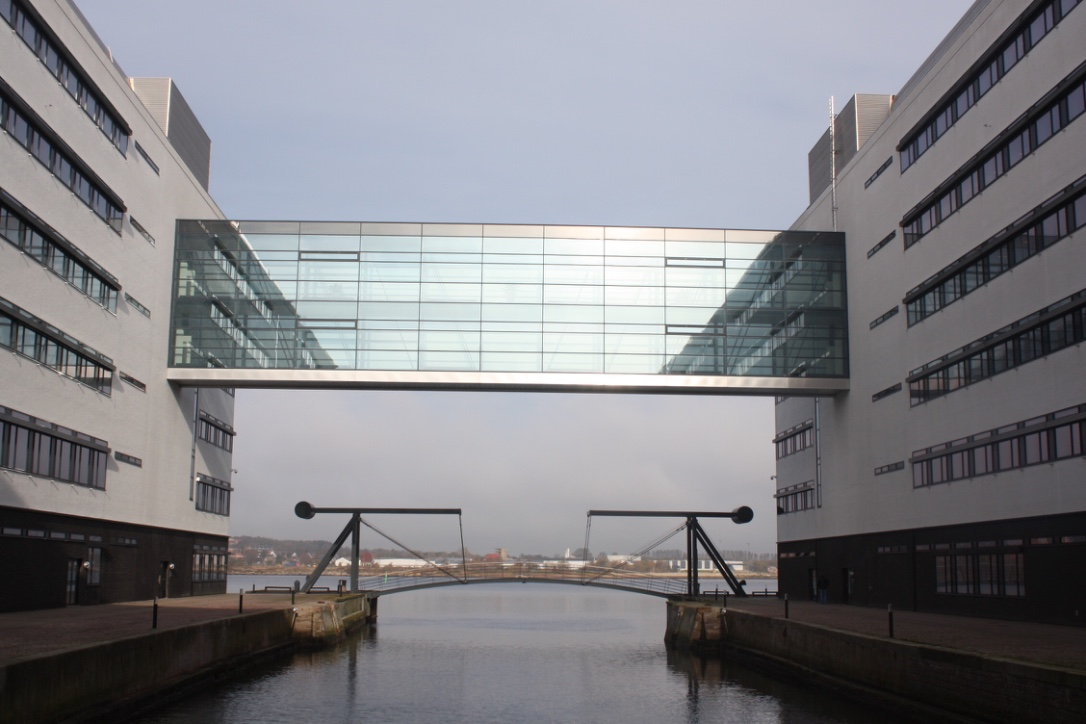
\includegraphics[width=1\textwidth]{billeder/KMDgangbro.jpg}

\vspace{2cm} 
\textsc{\Large P2 - Projekt \\
Gruppe B2-23 \\
Byggeri \& Anlæg 2\\
Aalborg Universitet\\
Den 23. maj 2016\\}
\end{flushright}

%\cleardoublepage												% Indsaetter tom side, saa naeste kapitel starter paa hoejre side (hvis noedvendigt)
%% Dette er LaTeX-versionen af titelbladet for TNB studenterrapporter
% Filen kræver:
% Universitetets logo:  AAU-logo-stud-UK eller AAU-logo-stud-DK
% Synopsis: En fil ved navn synopsis.tex

% Udarbejdet af: Jesper Nørgaard (jesper@noergaard.eu) 10. april 2012

\phantomsection
\pdfbookmark[0]{Titelblad}{titelblad}
\thispagestyle{empty}

\begin{minipage}[t]{0.48\textwidth}
\vspace*{-25pt}			%\vspace*{-9pt}

\includegraphics[height=4cm]{billeder/AAU-logo-stud-DK-RGB}
\end{minipage}
\hfill
\begin{minipage}[t]{0.48\textwidth}
{\small 
\textbf{Første Studieår v/ Det Teknisk-}\\
\textbf{Naturvidenskabelige Fakultet}  \\
Byggeri og Anlæg \\
Strandvejen 12-14 \\
9000 Aalborg \\
http://www.tnb.aau.dk}
\end{minipage}

\vspace*{1cm}

\begin{minipage}[t]{0.48\textwidth}
\textbf{Titel:} \\[5pt]\hspace{2ex}
Fundering af tilbygning af Strøybergs Palæ \bigskip

\textbf{Projekt:} \\[5pt]\bigskip\hspace{2ex}
P2-projekt

\textbf{Projektperiode:} \\[5pt]\bigskip\hspace{2ex}
Februar 2016 - maj 2016

\textbf{Projektgruppe:} \\[5pt]\bigskip\hspace{2ex}
B2-23	

\textbf{Deltagere:} \\[5pt]\hspace*{2ex}
Alexander Schacht \\\hspace*{2ex}
Emil Faber B.-S. \\\hspace*{2ex}
Hussein Al-Ali \\\hspace*{2ex}
Johnny Tuan N. \\\hspace*{2ex}
Jonas Damsbo \\\hspace*{2ex}
Mads Bjørndal N.\\\bigskip\hspace*{2ex}
Massir Thaafghan

\textbf{Vejledere:} \\[5pt]\hspace*{2ex}
Søren Dam Nielsen og Niels Agerholm




\vspace*{1cm}

\textbf{Oplagstal: 10} \\
\textbf{Sidetal: 118 } \\
\textbf{Appendiks: 33 } \\ 
\textbf{Afsluttet 18-12-2015}

\end{minipage}
\hfill
\begin{minipage}[t]{0.483\textwidth}
Synopsis: \\[5pt]
\fbox{\parbox{7cm}{\bigskipDette P1-projekt omhandler KMDs nordlige langt-spændende gangbro, som forbinder KMDs to hovedbygninger med hinanden. I kapitlet \textit{Beskrivelse af konstruktion}, beskrives KMDs gangbro detaljeret, med hvilke materialer den er lavet af samt dens dimensioner. I kapitlet \textit{Stål og dets egenskaber}, beskrives det anvendte stål, dets flydespænding samt dets tryk og træk styrker. I kapitlet \textit{Standarder og normer}, beskrives hvad Eurocodes, Dansk Standard, partialkoefficienter og Bygningsreglementet er. I kapitlet \textit{Laster} beregnes egen-, nyttelasten, vind- og snelasterne for KMDs gangbro. I kapitlet \textit{Statisk dokumentation} beregnes reaktionerne og de indre kræfter. Dernæst bevises det, at bæreevne er tilstrækkelig. Tilsidst konkluderes de opstillede problemstillinger i en besvarelse, hvor det munder ud i, at gangbroen er dimensioneret tilstrækkeligt.


\bigskip}}
\end{minipage}

\vfill

{\footnotesize\itshape Rapportens indhold er frit tilgængeligt, men offentliggørelse (med kildeangivelse) må kun ske efter aftale med forfatterne.}

% Rapportens indhold er frit tilgængeligt, men offentliggørelse (med kildeangivelse) må kun ske efter aftale med forfatterne.
% The content of the report is freely available, but publication (with source reference) may only take place in agreement with the authors.

%\cleardoublepage
%\chapter*{Forord}

Denne rapport er resultatet af det arbejde projektgruppen A408a, bachelor Byggeri og Anlæg på Aalborg Universitet, har lavet i P1-projektet på første semester. Rapporten er udarbejdet fra perioden d. 6. oktober til d. 18. december. Det overordnede emne for dette P1-projekt er; Aalborg, en by i stadig forandring, med underemnet; Analyse af bæreevnen af langt-spændende gangbro, hvor der er arbejdet med tekniske og kontekstuelle problemstillinger for udformningen af KMDs gangbro og eftervisning af dens bæreevne. Vi vil gerne takke vores vejleder, Jonas Bjerg Thomsen, for hans indsats, hjælp og gode samarbejde igennem hele projektperioden.

\textbf{Læsevejledning}

Rapporten udformet således, at der løbende kommer kildehenvisninger i teksten, som til sidst er uddybet i en litteraturliste. Kildehenvisningerne i denne rapport er lavet med Harvard metoden, som angives med: [Forfatterens efternavn/virksomhed, udgivelsesår]. Ved referering til en hjemmeside anvendes samme metode, dog skrives der i litteraturlisten hvornår den sidst blev set. I litteraturlisten er kilderne organiseret i en kronologisk rækkefølge. Hvis der er en kilde, som har samme forfatterefternavn og udgivelsesår, tilføjes et suffiks i form af et bogstav (a,b osv.), dette gøres, så det er muligt at kende forskel på kilderne. I selve litteraturlisten angives forfatter(e), titel, udgave, oplag, ISBN-nummer og forlag, hvor hjemmesider har forfatter(e) eller virksomhed, titel, internetadresse, årstal og besøgsdato. Figur- og tabel nummerering er opstillet i kronologisk rækkefølge. Det første tal i et figur- eller tabelnummer er kapitelnummeret, det andet tal er figurens eller tabellens navn. Et eksempel på dette kunne være den femte figur i kapitel tre, den vil blive nummeret som Figur 3.5. Figurer uden en kildehenvisning er udarbejdet af projektgruppen selv.



\phantom{Luft}

\phantom{Luft}

\begin{table}[H]
	\centering
		\begin{tabular}{c c c}
			\underline{\phantom{mmmmmmmmmmmmmm}} & \underline{\phantom{mmmmmmmmmmmmmm}} & \underline{\phantom{mmmmmmmmmmmmmm}} \\
			Alexander Schacht			& Emil Faber B.-S. 		& Hussein Al-Ali 			\\
			&&\\
			&&\\
			\underline{\phantom{mmmmmmmmmmmmmm}} & \underline{\phantom{mmmmmmmmmmmmmm}} & \underline{\phantom{mmmmmmmmmmmmmm}} \\
			Johnny Tuan N.			& Jonas Damsbo 		& Mads Bjørndal N. 	\\
			&&\\
			&&\\			
&\underline{\phantom{mmmmmmmmmmmmmm}} \\ 														
			& Massir Thaafghan
																		
		\end{tabular}
\end{table}
%\cleardoublepage

%%%% Indholdsfortegnelse (TOC) %%%%

\phantomsection													% Kunstigt afsnit, som hyperlinks kan 'holde fast i'
\pdfbookmark[0]{Indholdsfortegnelse}{indhold}					% Tildeler en klikbar bookmark til den endelige PDF
\tableofcontents*												% Indholdsfortegnelsen (kaldet ToC)

%\addtocontents{toc}{\protect\newpage}							% Fremtvinger sideskift i ToC hvis noedvendig (der hvor koden placeres)


\mainmatter														% Hovedindhold - nummereres fra side 1

%%%% Rapportindhold %%%% 										% Rapportindholdet boer IKKE indeholde broedtekst - KUN includede filer!

%% Indledende %%												% Opdel evt. i passende afsnit for overblikkets skyld

%\chapter{Indledning}



%\chapter{Problemanalyse}
Dette afsnit vil indeholde en argumentation for, hvad denne rapports grundlæggende emnevalg er samt en motivationsdel til rapporten, som er givet ud fra en undren over emnet. Til sidst vil metodevalget blive begrundet.  
 
\section{Initierende problem}
KMDs langt-spændende gangbro er en konstruktion, der er udformet som en gitterkonstruktion. Dette danner grundlag for en gennemgang af analytiske modeller og metoder, der anvendes til at bestemme konstruktionens stabilitet og dimensioner. Igennem tiderne har forkerte modeller og metoder betydet delvise eller totale kollaps for bygninger. For eksempel da Superarenaen i Ballerup kollapsede den 3. januar 2003  pga. fejldimensionering af bjælkerne og i vinteren 2009-2010 hvor der skete en sammenstyrtning af en stald pga. en dimensioneringsfejl i de bærende søjler. I dette projekt vil der forsøges at opnå en forståelse af de anvendte modeller og metoder til at eftervise en konstruktions bæreevne og hvordan den er sikret via beregningerne. Dette rejser en række interessante spørgsmål, som er opdelt i følgende punktform. 
 
 \begin{itemize}
 \item Hvad påvirker gangbroens konstruktion?
 \item Hvilke metoder anvendes ved bestemmelse af bæreevnen? 
 \item Hvordan sikres konstruktionerne i de benyttede last- og beregningsmodeller? 
 \end{itemize}
 
\section{Problemformulering}
Ved den initierende problemstilling blev der set på nogle interessante områder, som projektgruppen ønsker at eftervise med denne rapport. Dette munder ud i en konkret problemstilling, hvor metoden last-system-respons vil være oplagt at anvende til beregning eller eftervisning af konstruktionens stabilitet og dimensioner. Dette sikrer processen fra modeller og forudsætninger til virkeligheden. For at man nemmere kan tyde de opstillede problemer, opdeles det i følgende underpunkter.

\begin{itemize}
\item Hvilken type konstruktion er KMDs gangbro?
\item Hvorfor er stål egnet som byggemateriale?
\item Hvilke laster bliver gangbroen påvirket af?
\item Hvordan anvendes knudepunktsmetoden til at finde den samlede lastpåvirkning for gangbroen?
\item Er dimensionerne af profilerne i gangbroen tilstrækkelige?
\end{itemize}

\section{Problemafgrænsning}
I denne rapport er projektets fokus, hvilket grundlag der er for dimensioneringen af gangbroen. Dette munder ud i en statisk model, som består af relevante beregninger, som resulterer i hvorvidt dimensioneringen af stålprofiler er korrekt eller i så fald er overdimensioneret eller underdimensioneret. Igennem rapporten vil de relevante metoder blive brugt til at besvare problemstillingerne. Rapporten er udarbejdet, som et produkt af et P1-projekt indenfor det ingeniørvidenskabelige basisår. Dette resulterer i en tidsbegrænset proces, som har betydning for rapportens indhold og derfor er det nødvendigt at lave en afgræsning. Derfor vil nedenstående problemstillinger ikke blive taget i betragtning og vil dermed blive afgrænset fra rapporten:

\begin{itemize}
\item KMDs to hovedbygninger.
\item Aalborgs lokalplan for Sturhs Brygge.
\item Geotekniks analyse af byggegrunden. 
\item Det økonomiske aspekt indenfor byggeprojektet.
\item Gangbroens energi og indeklima.
\item KMDs begrundelse for opførelsen af gangbroen.
\item De indre vindkræfter.
\item De arkitektoniske overvejelser. 
\item De hensigtsmæssige ulykkeslaster og brandsikringen.
\end{itemize}

\section{Metodevalg}
P1-projektets metodevalg er baseret på, at rapporten vil beskrive KMDs gangbro ud fra en ingeniørs synsvinkel. Metoden behandler tre hovedpunkter, som kendes fra én metode, last-system-responsmetoden. Denne metode anvendes til overvejelser for gangbroens konstruktion. Projektet vil inddrage beregninger, som vedrører de forskellige laster. Det, som optager lasterne er gangbroens konstruktion, hvormed gitterkonstruktionen er systemet, som håndterer lasterne.  Responsen af gangbroen er herefter det interessante, hvor det kan sættes i sammenhæng med, om konstruktionen er tilstrækkelig dimensioneret. Der vil blive analyseret ud fra beregninger af de indre kræfter i gangbroen.

%Kontekstuelt%


%\chapter{Initierende problem}

\section{Initierende problem}

Geologien i et byområde har stor betydning for hvordan en by udvikler sig. Dette kan man i Aalborg se blandt andet ved virksomheders placering som Aalborg Portland. Limfjorden har også stor betydning for byudvikling, især når man ser fremadrettet hvor man forventer store vandstandsstigninger, grundet klimaændringer. Geologien er ikke det eneste der har betydning for byudvikling, urbanisering er også en stor faktor, da en tilstrømning af mennesker kræver en klar plan for hvor der skal bygges nyt, og hvor der skal bygges om. 


Kommunerne i Danmark skal have en plan for hvordan de skal udvikle sig fremadrettet. Aalborg Kommunes plan går ud på at omdanne Aalborg fra en industriby til en kompetenceby, et vidensbaseret samfund. Da Aalborg er blandt Danmarks største byer, kommer der mange nye mennesker til, dette kræver at Aalborg kommune har en plan for hvor der skal opføres nye boligområder og hvor gamle boligområder skal ombygges. Det initierende problem lyder således:


\textit{Hvordan har Aalborg udviklet sig som en by gennem tiden og kan geologien i området have betydning for byens udvikling.}


I de første kapitler af rapporten vil det initierende problem blive belyst, Aalborgs historiske og fremtidige byudvikling vil blive redegjort og analyseret, der vil blive undersøgt om geologien i området har betydning for Aalborgs udvikling og der vil komme en interessentanalyse om en eventuel tilbygning til Strøybergs Palæ.

\section{Metodeafsnit}
Dette er ikke skrevet endnu.

%\chapter{Geologisk historieundersøgelse}

\textbf{NB: i det følgende kapitel skal der ses bort fra de manglende figurer og de ikke fuldstændige figur referencer.}


I dette kapitel er der en analyse af de geologiske forhold i Aalborg, samt en redegørelse for de historiske forhold der har været medvirkende til dannelse af disse geologiske forhold. 
Kapitlet vil have fokus på den glaciale, den senglaciale og den post glaciale periode, og vil yderligere også redegøre for de kridt forekomster der findes i Aalborg. 

Størstedelen af den jord der findes i Aalborg i dag, har oprindeligt været en bjergart som gennem tiden er blevet forvitret og transporteret. Det er de forskellige forhold i de forskellige tidsperioder der har været medvirkende til at de forskellige jord aflejringer er sket. Disse forskellige forhold for de forskellige perioder vil blive beskrevet herunder:

\section{Den Glaciale periode}

Glaciale perioder omfatter de perioder hvor landskabet har været dækket af gletsjere. I Danmark findes der spor efter de seneste fire istider, herunder Menap-, Elster-, Saale- og Weichsel istiden. Mellem istiderne har isen været smeltet bort, disse perioder kategoriseres som interglaciale perioder. 

Der vil i dette kapitel kun fokuseres på den sidste glaciale periode, mere specifikt Sen Weichsel perioden som strækker sig fra ca. 25.000 år siden til ca. 9.500 år siden. I denne periode var Nordjylland nedfrosset og dækket af gletsjere, disse gletsjere har medbragt nogle forvitret materialer som bl.a. omfatter forvitrede og løsrevne klippestykker fra Skandinaviens fjelde, og medslæbte bløde jordarter. Disse materiale blev under is-transporten knust og sammenblandet.

Ved isens smeltning ville dette materiale enten udfaldet som en yderest usorteret substans, eller aflejre sig som velsorterede jordarter gennem en kort/lang transport forårsaget af isens smeltevand. Denne transporten kunne have forgået under, i eller udenfor isen. 

Den usorterede blanding som er en sammenblanding af ler, sand, grus og sten, betegnes som moræne. Herfra kan man opdele det i moræneler, morænesand osv. alt efter hvad der er karakteristisk. På samme måde inddeles smeltevandsaflejringerne efter kornstørrelser

Denne transport kan ses af figur X.X 
NOTE: Johnny scanner billede fra kort  


Som det fremgår omfatter glaciale aflejringer moræneler, morænesand, morænegrus og smeltevandsaflejringer i form af smeltevandssand og –grus. 

\section{Glaciale aflejringer i Aalborgområdet}
De glaciale aflejringer kan findes flere steder i Aalborgområdet som topografisk materiale, placeringen af disse kan ses af figur X.X 
NOTE: Johnny scanner kortet for mig, det er very nice (borat stemme)

Som det ses af figur X.X findes der smeltevandssand og –grus aflejringer som topografisk materiale syd for fjorden strækkende sig fra Sønder Tranders op over Øster Sundby og videre op mod Limfjorden. Desuden findes der en større ø bestående af smeltevandssand og –grus nord for fjorden som strækker sig op til Hvorup. 

De glaciale moræner findes i et meget begrænset omfang som topografisk materiale i Aalborgområdet, der ses dog en relativt større forekomst af moræneler nær Sønder Tranders, mens de resterende forekomster af moræneler forekommer relativt sporadisk i Aalborgområdet.
 
Den sidste del af Weichsel-istiden betegnes som den senglaciale periode. Denne periode strækker sig over en periode der går fra omkring 17.000 år siden 9.500 år siden, altså frem til afslutningen af Weichsel-istiden. Denne periode markerer en overgangs periode mellem den sidste istid og den nuværende interglaciale periode. 

\section{Den senglaciale periode}
Perioden er i høj grad karakteriseret af et klima der varierede mellem tundra lignende forhold med lav vegetation, og varmere perioder med en større fauna og et rigere dyreliv. Generelt for perioden er at klimaet blev varmere hvilket betød at Nordjylland og derfor også Aalborgområdet blev isfrit da gletsjerne smeltede bort som følge af det varmere klima. Denne bortsmeltning af isen medførte markante havstigninger og betød at Nordjylland blev dækket af et ishav. Dette ishav fik navnet Yoldia havet efter en ishavsmuslingen Portlandia (tidligere Yoldia) der levede i havet. Yoldiahavets højeste strandlinjer har ligget ca. 20 m over den nuværende havoverflade, derfor vil der kunne findes senglaciale aflejringer i kote 20. De højeste strandlinjer for resten af Nordjylland ses af figur X.X


NOTE: Indsæt Yoldiakort som Johnny sama scanner for mig. 


I den nordlige del af Nordjylland hvor der var tale om havaflejringer, har området været præget af et rigt dyreliv. Her er der først blev afsat et sandlag, kaldet Nedre Saxicava-sand, som er opkaldt efter den musling som har levet i havet. Efterfølgende er der blevet afsættet er lerlag, Yoldialer, som er opkaldt efter den førnævnte Portlandia musling. Til sidst afsluttes med en sandaflejring, Øvre Saxicava-sand.

Syd for Vendsyssel, og dermed Aalborgområdet, har forholdende været anderledes. Den største forskel ligger i, at lagene ikke indeholder muslinger eller andre dyrerester. Det vil sige, at de pågældende lag ikke er blevet afsat på bunden af et hav, men er blevet opbygget i et ferskvands eller brakvandsmijø. Udover det, så er det sandlag som danner underlag for Yoldia-leret ved Vendsyssel mere sammenhængende hvorimod ved Aalborgområdet optræder sandet mere tilfældigt. Den skalfrie Yoldia-ler  som befinder sig  i Aalborgområdet har man valgt at betegne som Aalborg-ler. Som det kan ses på figur X.X, så ligger dele af Aalborg lagende forholdsvis højt. Det betyder at forekomsten af leret i Aalborg også været let tilgængelig og det har senere haft stor betydning for det lokale teglværks- og cementindustri. 

\begin{figure}[H] 
\centering
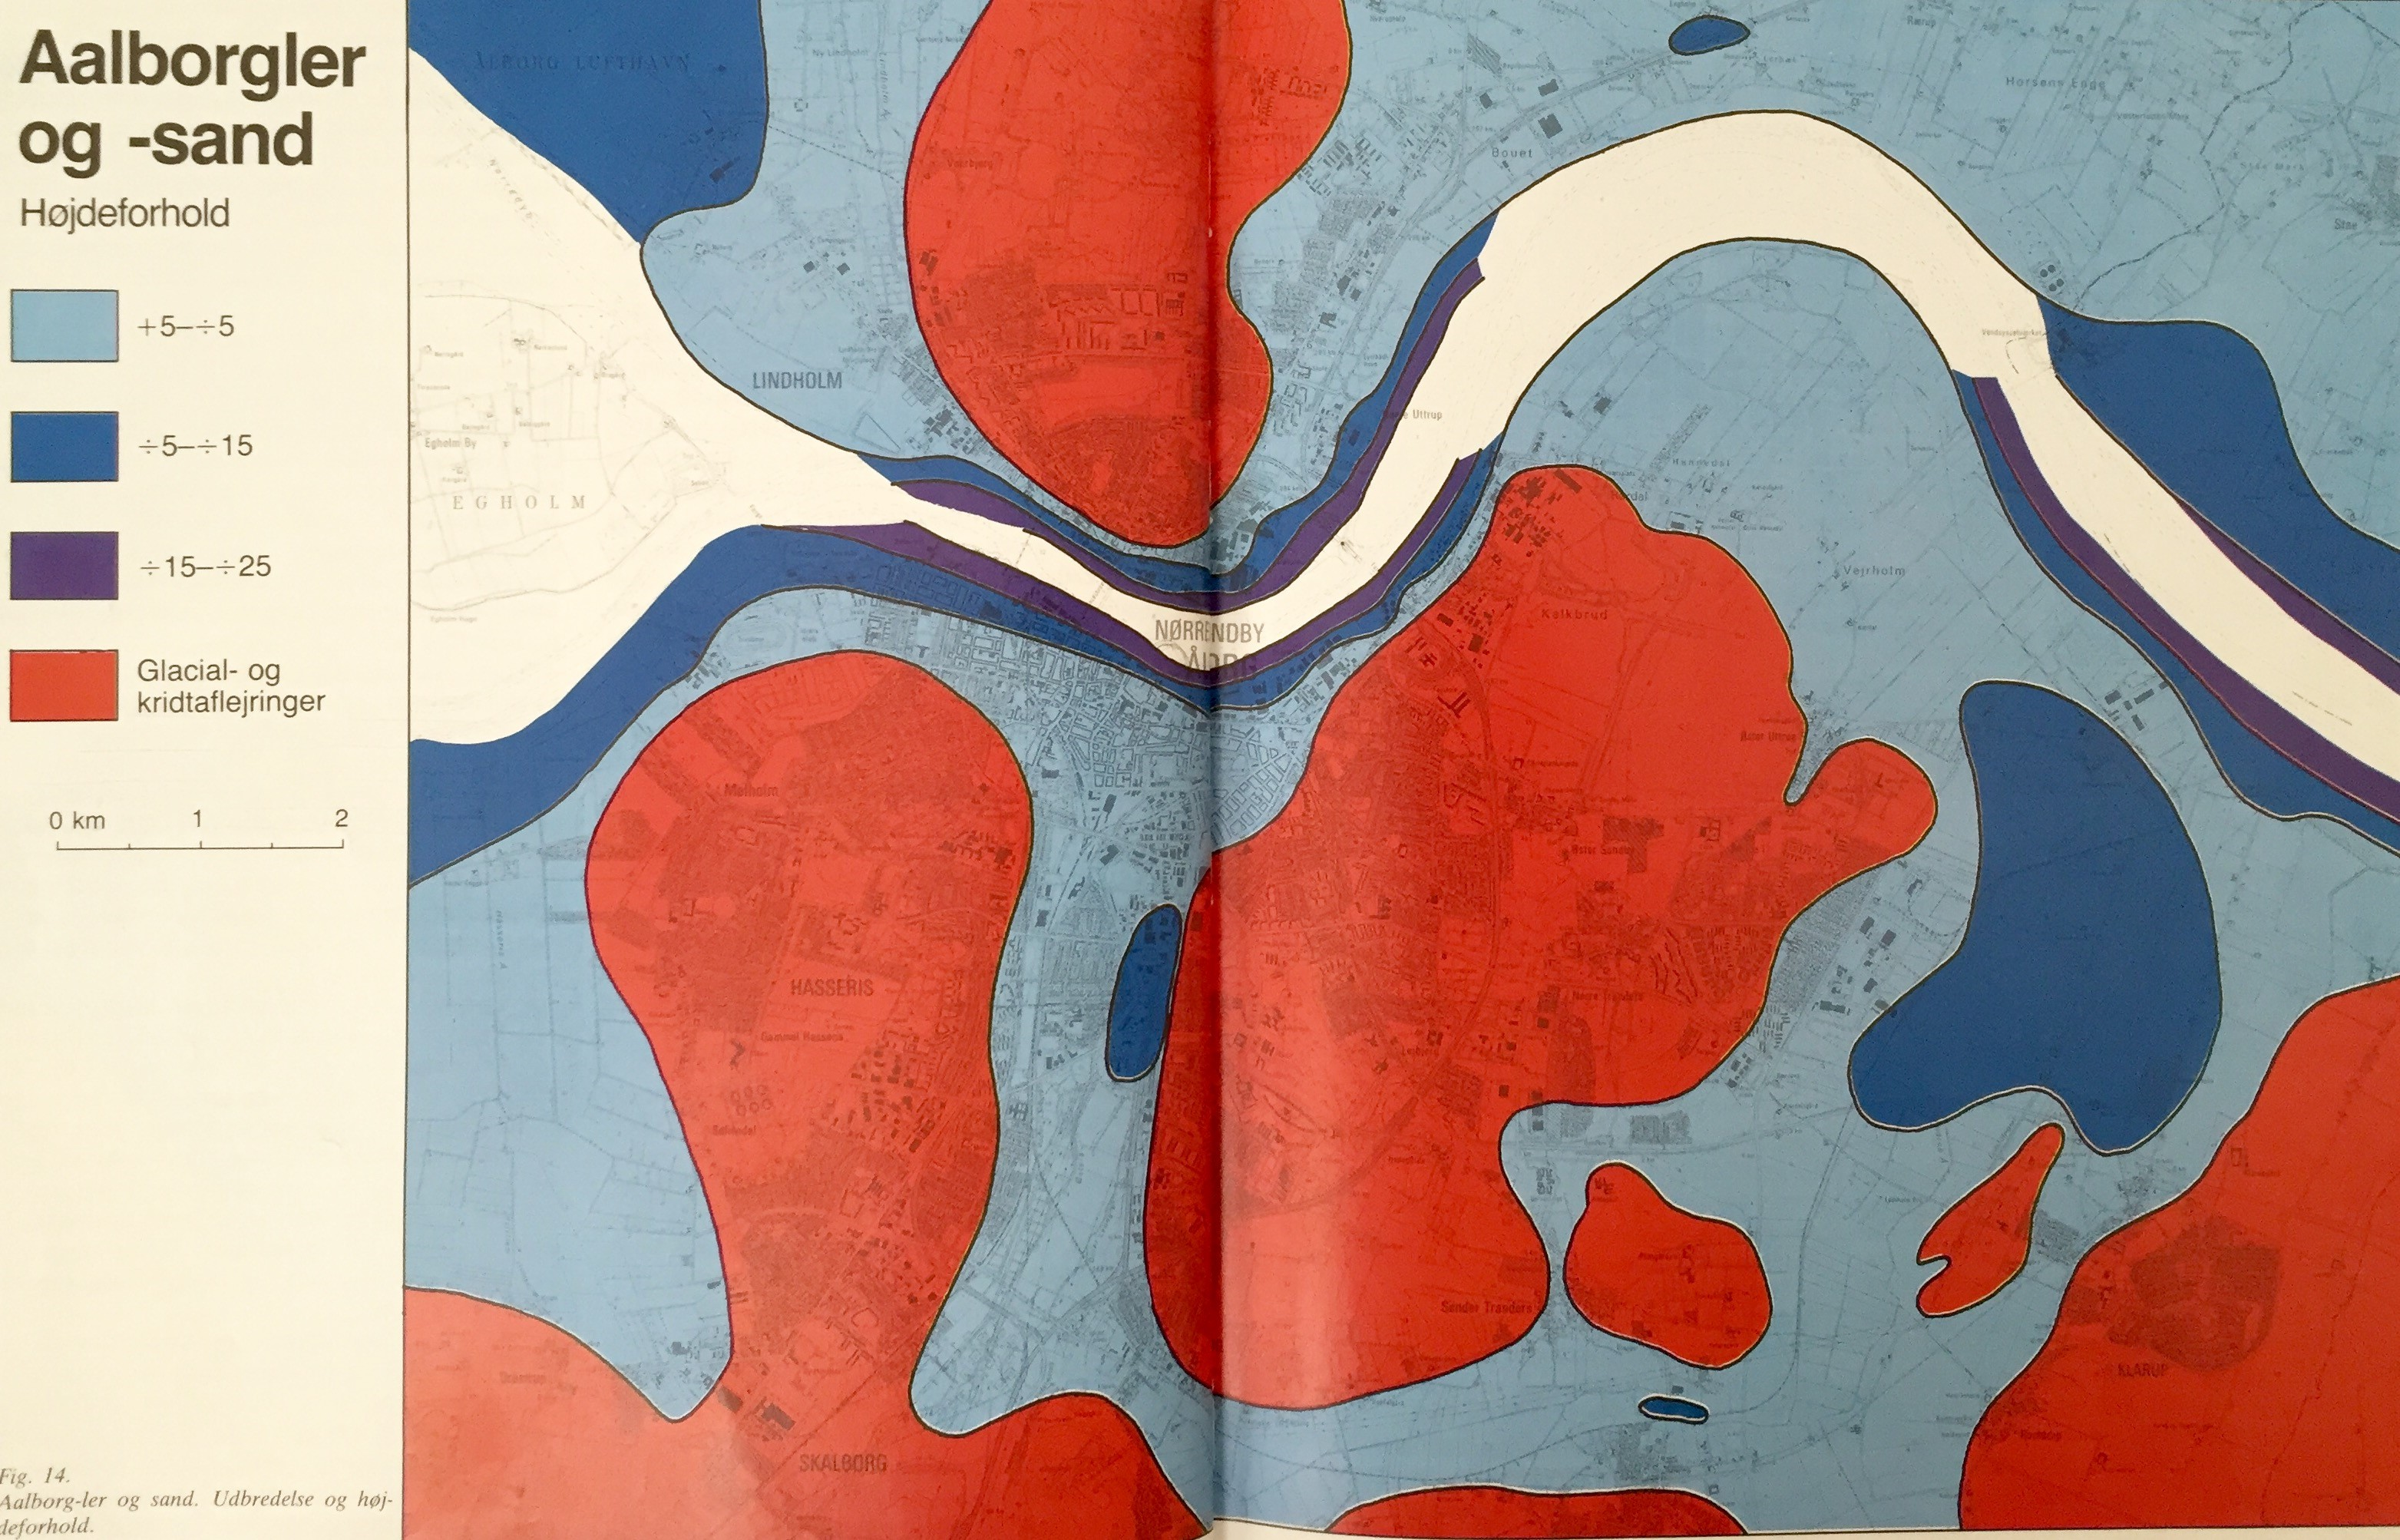
\includegraphics[width=0.90\textwidth]{billeder/GHU4}
\caption{Figuren viser forekomsterne af Aalborg-ler og -sand. Ved Limfjorden kan Aalborg-ler først findes 25 meter under fjordoverfladen.}
\label{fig:GHU4}
\end{figure}

Det ses at de senglaciale aflejringer typisk ligger lavt nær Limfjorden i Aalborg, dog ses det af Figur X.X (Det store kort med topografiske materiale) at Aalborg-leret findes som topografisk materiale i mindre områder langs Limfjordens syd- og nordlige side. 

Det ses også af kortet at det tilnærmelsesvis kan vurderes at det umiddelbare topografiske materiale der findes under Strøybergs palæ er Aalborg-ler altså en senglacial aflejring. Dette er imidlertid modstridende med den udleverede jordbundsundersøgelse, og derfor vil dette ikke blive brugt videre i rapporten. 

Efter den senglaciale periode fulgte den postglaciale periode, som startede for omkring 9.500 år siden og er endnu ikke afsluttet. Den postglaciale periode markere starten på den Holocæne epoke og Flandern – mellemistiden, som er den interglaciale periode vi i dag befinder os i. 

\section{Den Postglaciale periode}

Klimatisk set var de første ca. 2000 år af den postglaciale periode koldere end det nuværende klima, men varmere end det klima der havde domineret den senglaciale periode. For omkring 7000 år siden begyndte klimaet i højere grad at minde om det klima der ses i dag. Disse klimatiske har betydet at et stadig mere udbredte skovområder i Nordjylland, dette ses også ved at der flere steder i Aalborg er dokumenteret tørv materiale er påvist. Disse tørvforekomster ses af Figur X.X

NOTE: Scan billede på side 28 og skriv noget med at de er markeret med ringe.

De før omtale klimatiske forbedringer betød også at for omkring 7.500 år siden medførte gletsjer smeltninger i det nordlige Skandinavien at Aalborg igen var dækket af hav. Havet fik navnet Stenalderhavet da dets maksimale udbredelse lå i stenaldertiden. Der var denne gang ikke tale om et ishav, men et hav der minder meget om det der findes i Aalborg området i dag. De højeste forekommende strandlinjer for Stenalderhavet lå ca. 6-8 meter højere end det nuværende hav niveau, altså må de højeste forekommende postglaciale aflejringer forventes at kunne findes i kote 8. De resterende højeste standlinjer for Nordjylland kan ses af Figur X.X  

NOTE: Indsæt figuren fra side 47

De hyppige postglaciale aflejringer omfatter saltvandsler og saltvandssand. At den postglaciale periode er den senest forekommende periode og derfor også de senest aflejrede materialer ses også af Figur X.X (Det kvartærologiske kort) hvor af det ses at de postglaciale aflejringer er de mest udbredte topografiske materiale i Aalborg området, hvor de forekommer, både på den nordlige- , såvel som den sydlige side af Limfjorden. Det er dog værd at bemærke at manglende boringer i området umiddelbart syd for Limfjorden, betyder at dette område ikke er kortlagt. Det må dog anses som værende sandsynligt at de postglaciale aflejringer vil være hyppigt fundne som topografisk materialer i dette område. 

\section{Opsummering}

Som det ses af ovenstående kapitel findes der aflejringer fra alle tre analyserede perioder i Aalborg, både som topografisk materiale, men også dybere i jorden. I forhold til at dette projekt omhandler funderingen af tilbygning, anses det som værende relevant at se på de forskellige aflejringers egnethed som funderingsmateriale. 
Figur X.X viser et skema over de forskellige aflejringer fra de forskellige perioder, der kan findes i hele Danmark. 

NOTE: Indsæt figur fra side 43 i geobogen. Skriv figur tekst der forklare betydningen af 

Overordnet set ses det at desto ældre aflejringen er, desto bedre er styrke- og deformationsegenskaberne, og ydermere ses det også at muligheden for sætninger aftager med alderen af aflejringerne. 
Derfor ses det at de glaciale aflejringer hverken giver anledning til sætninger og har desuden styrke- og deformationsegenskaber der klassificeres som værende ”Meget gode – Gode”. Den generelle forklaring på dette, er at disse aflejringer har været hårdt sammenpresset af gletsjer masserne i de glaciale perioder og har derfor været belastet i en udstrækning der må anses som værende urealistisk at en bygning eller anden konstruktion vil nå. 

I takt med at styrke og deformationsegenskaberne falder op mod den post glaciale periode, stiger muligheden for sætninger også, og det må derfor vurderes at de post glaciale aflejringer er de mindst gunstige funderingsmateriale af de tre analyseret perioder. 

En anden bemærkelsesværdig ting der ses af figur X.X (den der står lige oven over) er det faktum at organiske aflejringer som tørv og gytje begge har ugunstige styrke- og deformationsegenskaber. En lignende udvikling ses i de faldende styrke og deformationsegenskaber fra de glaciale aflejringer til de sen glaciale aflejringer, hvor de klimatiske forbedringer, som tidligere nævnt, har givet anledning til en større fauna og et rigere dyreliv, og derfor også en øget mængde organisk materiale i periodens aflejringer generelt. 

For at sætte de forskellige perioders aflejringer i forhold til Strøybjergs Palæ, kan dette gøres med et Skematisk snit Nordjylland.


Det har ikke været muligt nøjagtigt at fastlægge koten for de glaciale aflejringer, mens at koten for både de sen glaciale aflejringer og de post glaciale aflejringer er fastlagt ud fra de tidligere benævnte maksimale strandlinjer for henholdsvis Yoldiahavet og Stenalderhavet. 
Strøybjergs Palæ ligger i Kote 2.5 og vil ud fra det ovenstående skematiske snit af Nordjylland derfor både skulle funderes i post- og sen glaciale aflejringer såvel som glaciale aflejringer. 

Med de relevante geologiske forhold i Aalborg området fastlagt er der skabt et adækvat billede den jord der skal funderes i ved opførelsen af en udbygning til Strøybergs Palæ. 

Udover at påvirke valget af funderings metode og byggeriet generelt, har de geologiske forhold i Aalborg også påvirket Aalborgs byudvikling. Udover de analyseret aflejringer fra den glaciale periode, samt den sen- og post glaciale periode, findes der i Aalborg også aflejringer af Skrivekridt der stammer tilbage fra den øvre kridttid. Disse aflejringer er flere steder højtliggende og danner tre større kridtøer. Disse kridtøer ses herunder af Figur X.X

\begin{figure}[H] 
\centering
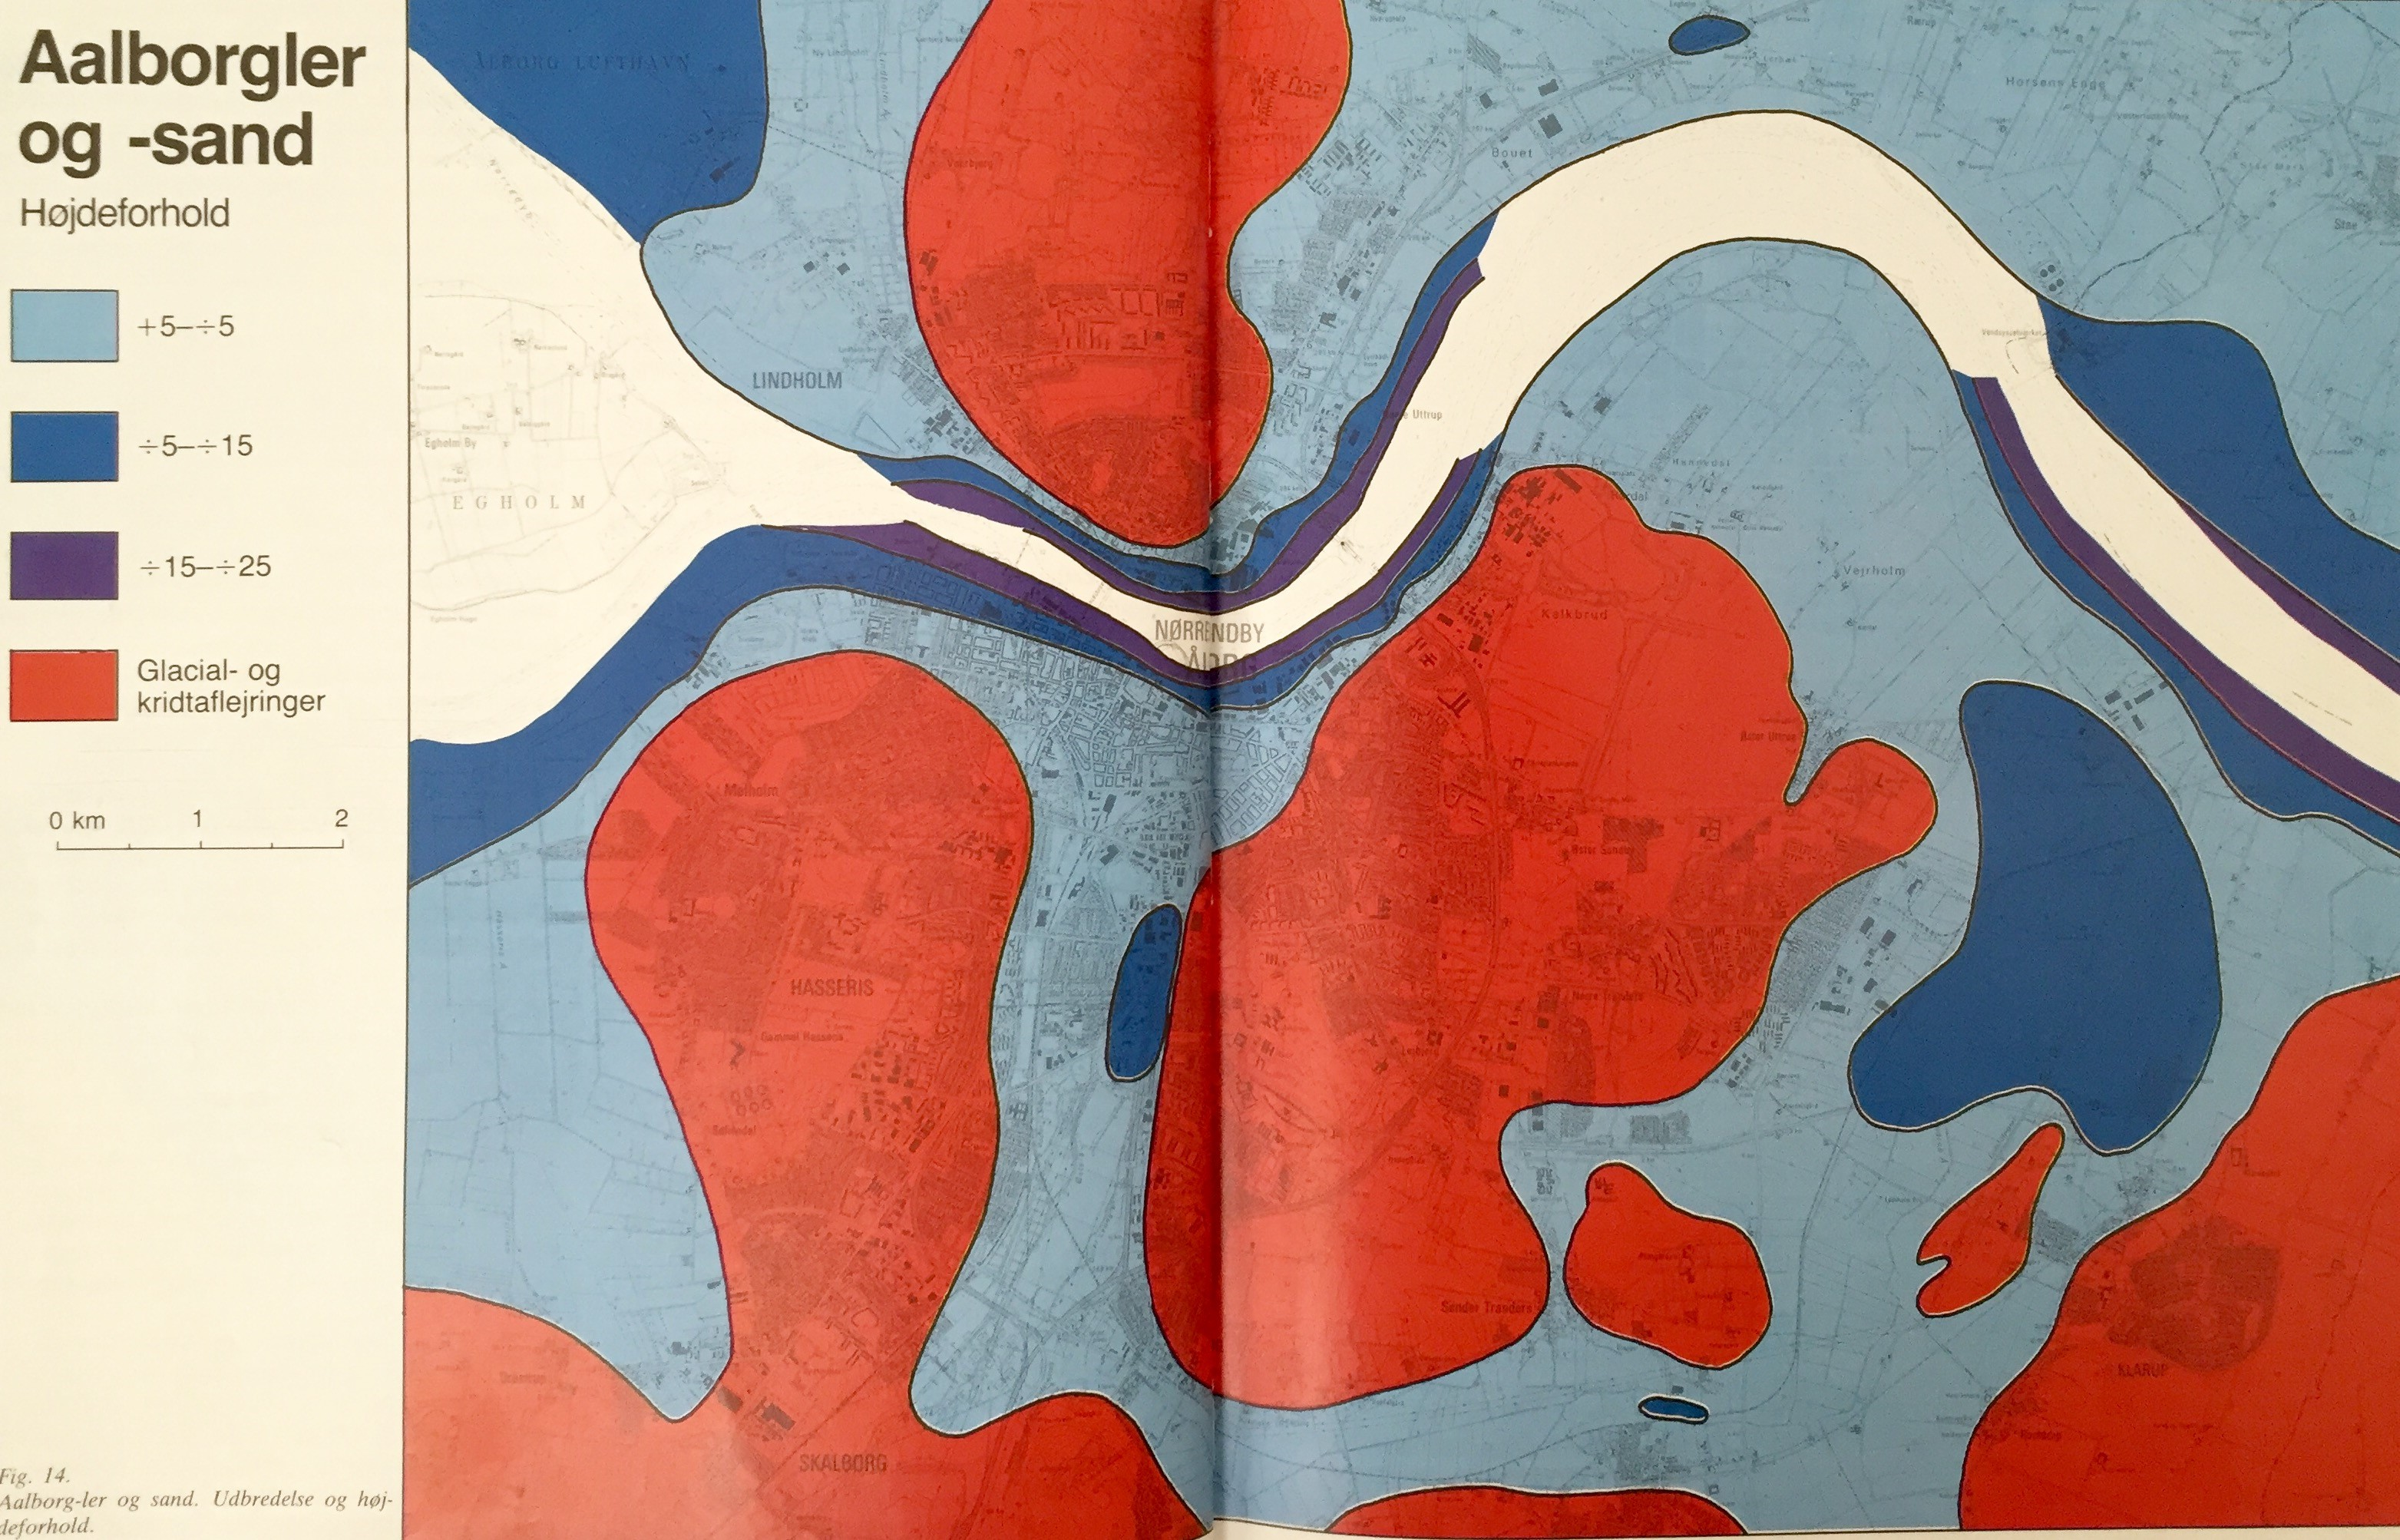
\includegraphics[width=0.90\textwidth]{billeder/GHU4}
\caption{Figuren angiver højden af kridtoverfladerne. De blåfarvede områder ligger under kote 0. De gule områder ligger højere end kote 0, og udgør de omtalte kridtøer..}
\label{fig:GHU2}
\end{figure}

Cement består af to primære komponenter, henholdsvis kalk og ler. Begge findes i jorden i Aalborg, og denne forekomst af Skrivekridt og det førnævnte Aalborg-ler har påvirket at der i den sidste del af 1800-tallet opstod en voksende cement industri i Aalborg, der i høj grad fungerede som dynamo for både byudviklingen og Aalborgs industrielle udvikling. Der findes stadig spor efter denne cement industri i Aalborg i dag i form af Aalborg Portland.

Aalborg er i dag gået fra en industriby til en kompetence by, og denne udvikling samt de visioner og nuværende tiltag Aalborg Kommune har, vil blive beskrevet og analyseret i det næste kapitel.   





%\chapter{Jordbundsundersøgelse}
I dette kapitel vil jordbundsundersøgelser blive beskrevet. Der vil blive lagt fokus på hvad en jordbundsundersøgelse er og hvorfor det er vigtigt at lave dem i forbindelse med fundering af en konstruktion.

En jordart er betegnet som et materiale, der består af løse mineralske- og organiske korn. Inden for geoteknik og ingeniørgeologi har det vist sig at være hensigtsmæssigt at arbejde med en række udvalgte jordarter. Hver jordart er opbygget af bestemte elementer og set fra en geologisk side, så er hver en jordart dannet på en bestemt måde. Disse jordarter indeholder nogenlunde defineret geotekniske egenskaber som mere eller mindre er forskellige fra jordart til jordart. Eksempelvis er der en kæmpe forskel på nogle af de danske jordarter som skrivekridt, gytje og moræneler. 

Man skal have et indblik i hvordan jordarterne er på en byggeplads, for at kunne have til kendskab om hvordan fundamentsunderlaget vil reagere på den dimensioneret konstruktion/bygning. Hvis jorden på to forskellige byggepladser består af samme jordart, så burde de reagere og opføre sig på samme måde. Hvorimod, hvis det er på samme byggeplads med to adskilte jordarter, så vil opførslen af jorden være forskellige. 

En jordbundsundersøgelse er en fysisk eller kemisk undersøgelse af jordforholdet for det omhandlende område. Det er en række jordarter, som man finder under jorden via jordbundsundersøgelsen. Det kan eksempelvis være ler, silt eller sand. I en geoteknisk undersøgelse oplyses jordbund-, miljø- og grundvandsforholdene på en byggeplads, så en konstruktion kan dimensioneres sikkert. En jordbundsundersøgelse deles i tre hovedtyper: indledende undersøgelser, projektundersøgelser og kontrolundersøgelser. 

Den første typeform, som er den indledende undersøgelse, er det vigtigt at have kendskab til jordens historie samt type. Det er en gennemgang af jorden ved hjælp af boringer. 

Den anden typeform, som er projektundersøgelsen, er det vigtigt at have hensigt til tre dele. Placerings-, parameter- og optimeringsundersøgelser. Man starter med at udføre nogle undersøgelser ved hjælp af boringer for at vurdere funderingsforholdene, for at kunne bestemme om det er hensigtsmæssigt at konstruktionen bliver placeret på grunden. Dernæst oplyses styrkerne af jorden ved hjælp af nogle feltforsøg. Det giver svar på jordlagets styrke samt deformationsegenskaber. Man går derefter videre til boringernes dybde i jorden, for at kunne aflæse jordens sammentrykkelighed og gennemstrømmelighed. Optimeringsundersøgelsen skal man aflæse og beregne på om det er økonomisk at optimere funderingsprojektet. 


\begin{figure}[H] 
\centering
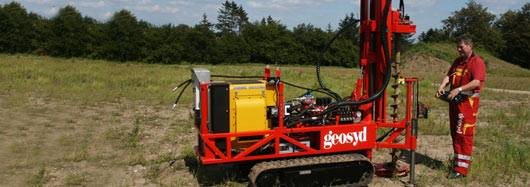
\includegraphics[width=0.50\textwidth]{billeder/Jordbund1}
\caption{Grafik af Aalborgs vækstakse}
\label{fig:Jordbund1}
\end{figure}




Eftersom de fleste øvre jordlag ikke kan holde til vægten af en bygning, bliver man nødt til at finde ud af hvad jorden består af, på en måde som funktion af dybden. Her er der altså tale om de tre jordforhold, Gl, Sg eller Pg. Nogle steder forholder det sig sådan, at jo længere ned man kommer, jo tættere og hårdere vil jorden være. For at fastslå den dybde hvor jorden kan bære og ikke vil sætte sig, er det nødvendigt at foretage jordbundsundersøgelser. 

I vores specifikke tilfælde har vi med en bygning at gøre, som ligger i relativ nærhed af vand. I nærheden af vand varierer jordtyperne meget, og grundvandsspejlets dybde får stor betydning for funderingstypen, samt størrelsen. Foruden dette varierer jordtyperne også meget i nærheden af vand, hvilket fremmer nødvendigheden af en dybdegående jordbundsundersøgelse. Desuden kan der i nærheden af vand skabes opdrift i jorden, da denne er lettere end vandet, hvilket vil skubbe på fundamentet nedefra. Herfor vil det være vanskeligere, uden en jordbundsundersøgelse, at sige med sikkerhed hvor det bærende lerlag befinder sig.




%\chapter{Byudvikling}
Dette kapitel handler om byudvikling i Aalborg. I kapitlet bliver Aalborgs udvikling fra en købsstad til en industriby til en kompetenceby beskrevet. Kommuneplaner generelt og  Aalborgs kommuneplan bliver beskrevet, hvor der bliver lagt særligt fokus på Vækstaksen. Lokalplanen for området hvor Strøybergs Palæ står bliver også beskrevet.

\section{Aalborgs udvikling til kompetence by}
Aalborg har i de seneste årtier været under stor udvikling fra at være en industriby, til at blive en videns- og uddannelses by.  Gamle industriområder, som en gang kendetegnede Aalborg, bliver i dag omdannet til nye boliger, kontorer, kultur og uddannelsessteder.

Byen Aalborg blev grundlagt tilbage i vikingetiden. Området var attraktivt da det havde gode havnemuligheder ud til Limfjorden. Byen blev i begyndelsen primært brugt som midtpunkt for markedspladser og værksteder. På grund af dette, var det ikke stor udvikling i byen, idet byen kun blev brugt som en form for samlingssted og ikke fast bosættelse. Det vides ikke sikkert hvornår Aalborg fik tildelt købstadsrettigheder men man ved, at byen begyndte at udvikle sig kraftigt fra ca. 1350 og frem. Dvs. at det højst sandsynligt er omkring denne periode, at byen fik tildelt købstadsrettigheder. Byens primære økonomi lå i salget af sild og korn. I 1600-tallet havde Aalborg stort set monopol på korneksport fra hele Vendsyssel og omkring Limfjorden. Byens købmænd tjente især stort på eksport til Norge og Tyskland.

I 1700-tallet oplevede Aalborg et fald i salget. Byen var stadig blandt de største i Danmark, men sildefiskeriet og korneksporten var ikke lige så attraktivt, som det havde været. Dette blev forværret med tabet af Norge i 1814, hvilket medførte at byen mistede vigtige handelsmarkeder.

På dette tidspunkt ligger Aalborg på sit laveste i en længere periode. I 1830’erne blev der etableret nye industrivirksomheder (heriblandt forløberen til De Danske Spritfabrikker), som var med til at opveje de økonomiske tab. Dette er således begyndelsen på Aalborgs bevægelse hen imod at blive en industriby, som i slutningen af 1800-tallet for alvor tog fat, som konsekvens af industrialiseringen, som bredte sig i hele Danmark i denne periode. Det var med udviklingen af dampmaskinen, at den industrielle revolution tog fat. Aalborg blev hjemsted for mange store virksomheder, specielt cementfabrikker, heriblandt Aalborg Portland, som nød godt af de store mængder kridt i Aalborgs undergrund og den nærliggende havn for transport. Disse industrivirksomheder satte for alvor gang i den industrielle udvikling i byen og medførte, at Aalborg gennem 1900-tallet var en udpræget arbejderby. Byen blev kendt som ”byen med de rygende skorstene”. 

Aalborg er i dag under omdannelse fra at være industriby til at være en kompetenceby. Siden 1960’erne og -70’erne, da henholdsvis Aalborg Seminarium og Aalborg Universitet blev grundlagt, har industrivirksomheder haft dalende betydning for byen. I slutningen af 1990’erne ombyggede man mange gamle industriområder til kontorer og boliger, pga. et stigende behov for dette. Ved år 2000 var op mod 60 procent beskæftiget inden for service- og uddannelseserhverv. På dette tidspunkt var det kun de mest veletablerede industrivirksomheder, som blev stående, mens mindre industrivirksomheder flyttede væk. Ved slutningen af 00’erne ses den største udvikling i form ombygningen af havnefronten øst for Limfjordsbroen, Kraftværket Nordkrafts omdannelse til kulturbygning og et stigende antal ungdomsboliger. I 2014 lukkede De Danske Spritfabrikker efter at være solgt til et Norsk selskab, som flyttede produktionen til Norge. Bygningen som nu står tilbage, skal efter planerne, omdannes til en international kunst- og kulturby.


\section{Kommuneplaner og Aalborgs kommuneplan}
En kommuneplan, er en kommunes overordnede plan for kommunens fremadrettede udvikling inden for de næste 12 år. Alle Danmarks kommuner har pr. lov, krav på, at have en kommuneplan. Det er kommunernes byråd, som står for at lave kommuneplaner. Kommuneplaner handler om hvordan erhverv, boliger og diverse servicefunktioner skal placeres i forhold til hinanden. En kommuneplan skal også vise en kommunes plan for trafikaflastning, det åbne land, skov områder, grønne områder mm. Byrådene, som laver kommunaplanerne, kan ikke gøre lige præcis som de vil, planerne skal overholde planloven. Kommuneplanerne er ikke direkte bindende for borgerne i kommunerne, f.eks. er grundejere ikke forpligtede til at overholde planen, dog siger planlovens §12, stk. 1, at kommunalbestyrelsen har pligt til at forsøge at få kommuneplanen gennemført. En kommuneplan indeholder følgende:

\begin{description}
\item [Hovedstruktur] er den overordnede, strategiske og sammenfattende fysiske plan for kommunen. Hovedstrukturen fastlægger de overordnede mål for udviklingen indenfor de enkelte områder og kommunen.
\item [Retningslinjer] udgør rammerne for kommuneplanen og kommunens administration af planlovens landzonebestemmelser og anden lovgivning indenfor bygge-, natur- og miljølovgivning.
\item [Kommuneplanrammer] styrer den overordnede anvendelse af kommunens arealer og danner rammer for indholdet af nye lokalpaner. Rammedelen er bygget op af bybeskrivelser, der beskriver udviklingen i kommunens byer og bydele, samt andre geografiske områder. Borgerne i kommunerne skal ikke direkte overholde kommuneplanrammerne, men de skal overholde de lokalplaner som bliver lavet ud fra kommuneplanrammerne.
\item [Bilag og tilhørende planredegørelse] beskriver forudsætningerne for ændringer i den konkrete planlægning. 
\end{description}

\subsection{Vækstaksen som byens motor}
Aalborgs fremadrettede udvikling skal være en målrettet og fokuseret byvækst, som skal ske i en vækstakse som strækker sig fra lufthavnen i nordvest til havnen i øst. Vækstaksen er vist på Figur \ref{fig:Vaekstakse1}

\begin{figure}[H] 
\centering
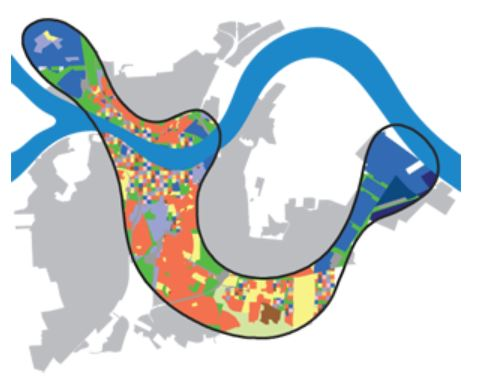
\includegraphics[width=0.50\textwidth]{billeder/Vaekstakse1}
\caption{Figuren viser den vækstakse som Aalborg primært skal udvikle sig i.}
\label{fig:Vaekstakse1}
\end{figure}

Kommunen vil have en koncentreret udvikling i denne vækstakse, hvilket betyder at offentlige og private investeringer skal koncentreres i vækstaksen, så synergier opstår og byen styrkes i fremtiden. I vækstasken skal der være tilbud og plads til alle behov og aldersgrupper, med hensyn til bolig, transport, natur, indkøb og fritidsinteresser. Vækstaksens endepunkter ved lufthavnen i nordvest og ved havnen i sydøst, skal udvikles som attraktive trafikbaserede erhversområder med gode forbindelser til resten af verden. Vækstaksen skal opnå storbykarakter, som kan tiltrække turister og fastholde både studerende og vidensarbejdere fra både ind- og udland. Det er vigtigt for vækstaksen at havnefronten, Karolinelund, Godsbanearealet, Eternitten, det østlige Aalborg, de bynære erhversarealer mm. skal færdiggøres og videreudvikles, da det skal sikre momentum og skabe attraktive og bæredygtige levevilkår

På Figur \ref{fig:Vaekstakse2}  er de udviklingsområder i vækstaksen med store potentialer for yderligere udvikling af Aalborg markeret. De markarede områder kan bidrage til udvikling af byen i form af boliger, arbejdspladser og styrkede grønne arealer. Nem og hurtig tilgængelighed i vækstaksen ligger til grund for udviklingen, idet målet med udviklingen er en styrket, bæredygtig udvikling kombineret med øget fremkommelighed.

\begin{figure}[H]
\centering
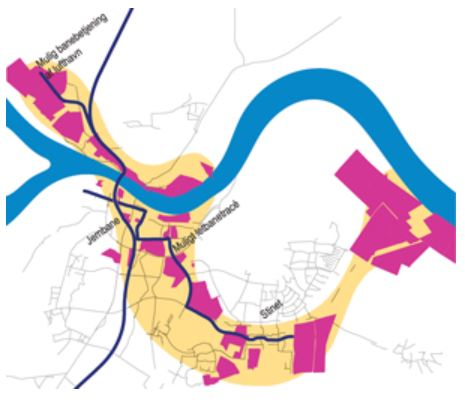
\includegraphics[width=0.50\textwidth]{billeder/Vaekstakse2}
\caption{Figuren viser de områder (markeret med lilla) som Aalborg Kommune primært vil have at Aalborg udvikler sig omkring.}
\label{fig:Vaekstakse2}
\end{figure}

Mobilitet er rygraden i vækstaksen, hvilket betyder, at det skal være let og hurtig adgang mellem centrale funktioner som f.eks. rekreative områder. Områderne omkring  knudepunkterne, vist på Figur \ref{fig:Vaekstakse3}, skal i særlig grad fortættes. Der skal sikres meget gode muligheder for at skifte mellem diverse transportformer, indkøb, service og bosætning, samt adgangsforholdene til knudepunkterne skal styrkes. Der skal på samme tid være en sammenhæng mellem vækstaksens vestlige og østlige endepunkter og byens centrum. 

\begin{figure}[H] 
\centering
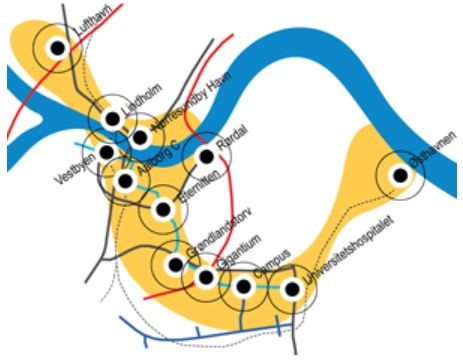
\includegraphics[width=0.50\textwidth]{billeder/Vaekstakse3}
\caption{Figuren viser de knudepunkter i Aalborgs vækstakse som der primært skal fortættes omkring. Infrastrukturen skal være særlig god i disse knudepunkter.}
\label{fig:Vaekstakse3}
\end{figure}

Kompetencebyen i Aalborg skal videreudvikles, dette gøres ved, at uddannelsesinsitutioner og ungdomsbolier koncentreres i vækstaksen. De mange studerende er med til at skabe liv i byen og hjælper med at lave en særlig oplevelseszone i centrum af Aalborg. Vækstaksen skal hjælpe Aalborg med at skabe et internationalt præg, som kan tiltrække udenlandske forskere, studerende og vidensarbejdere. Aalborgs Universitets Campus i Aalborg Øst skal udvikles til et regionalt midtpunkt med et meget levende studiemiljø og med diverse vidensvirksomheder.


\begin{figure}[H] 
\centering
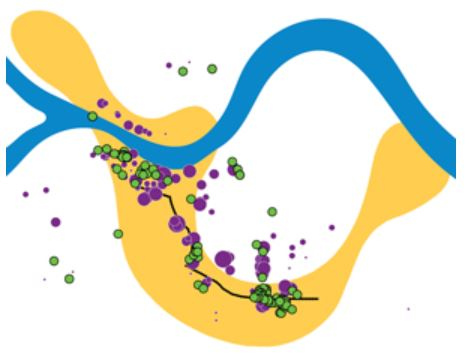
\includegraphics[width=0.50\textwidth]{billeder/Vaekstakse4}
\caption{Figuren viser de områder i Aalborgs vækstakse hvor der i særlig grad er og skal bygges ungdomsboliger, uddannelsesinstitutioner og vidensvirksomheder}
\label{fig:Vaekstakse4}
\end{figure}



\subsection{Byudviklingsprincipper for Aalborg}
Et af hoved byudviklingsprincipperne for Aalborgs kommuneplan er, at byen først og fremmest skal udvikles indenfor de eksisterende grænser, ved hjælp af fortætning og byomdannelse. Denne udvikling skal så være koncentreret særligt i vækstaksen. Sammen med fortætningen af byen skal der også udvikles en række grønne nærområder, så byen opnår en høj levekvalitet. Det er vigtigt for Aalborg, at byudviklingen tager hensyn til fjorden og landskabet ved Aalborg. På Figur \ref{fig:Byudviklingsprincipper1} ses byudviklingsprincipperne for vækstaksen.

\begin{figure}[H] 
\centering
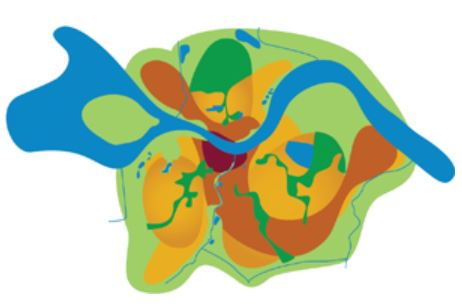
\includegraphics[width=0.50\textwidth]{billeder/Byudviklingsprincipper1}
\caption{Figuren viser Aalborg Kommunes vision for Aalborg.}
\label{fig:Byudviklingsprincipper1}
\end{figure}

I Aalborgs kommuneplan bliver der også lagt stor vægt på at sikre byen mod klimaændringer i fremtiden. I fremtiden forventes der mere nedbør og at vandstanden i havene stiger. Da fjorden løber igennem Aalborg, er Aalborg særligt udsat for fremtidige oversvømmelser. I klimastrategien betyder dette, at ved alt byggeri under kote 2,5m foretages der en klimasikring. Aalborg Kommune vil udarbejde en klimatilpasningsplan for hele kommunen, som skal være baseret på en kortlægning af oversvømmelsesrisici. For yderligere at sikre byen mod fremtidiger oversvømmelser, skal byen som udgangspunkt ikke udvikle sig længere mod de lavtliggende områder. Aalborg Kommune sigter efter at anvende de forøgede vandmængder rekreativt i byen. På Figur \ref{fig:Byudviklingsprincipper2} ses worst-case scenario for oversvømmelse i Aalborg-området 

\begin{figure}[H] 
\centering
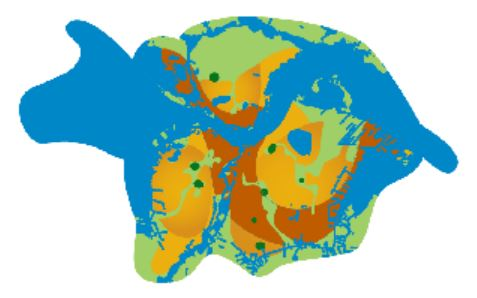
\includegraphics[width=0.50\textwidth]{billeder/Byudviklingsprincipper2}
\caption{Figuren viser worst-case scenario for oversvømmelse i Aalborg, når fjordens vandstand stiger.}
\label{fig:Byudviklingsprincipper2}
\end{figure}

Mobilitet skal ligge til grund for byens fremtidige udvikling, hvor især de bløde trafikanter skal prioriteres i midtbyen. I Aalborg skal der være stort fokus på bæredygtigt transport. Vækstaksen skal medvirke til at skabe et behov for en letbaneforbindelse, der skal bygges en tredje Limfjordsforbindelse og opføres en paralleltunnel. Der skal også laves en banebetjening til lufthavnen. På Figur \ref{fig:Byudviklingsprincipper3} ses mobilitetsplanen for Aalborg.

\begin{figure}[H] 
\centering
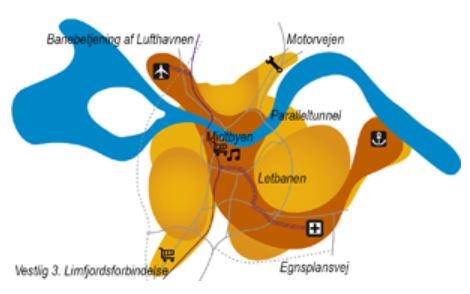
\includegraphics[width=0.50\textwidth]{billeder/Byudviklingsprincipper3}
\caption{Figuren viser Aalborg Kommunes mobilitetsplan for Aalborg, hvor blandt andet en letbaneforbindelse og en 3. limfjordsforbindelse indgår.}
\label{fig:Byudviklingsprincipper3}
\end{figure}

I perioden 2012-2024 viser Aalborg Kommunes befolkningsprognose, at der kommer en tilvækst på cirka 7000 borgere i Aalborg. Behovet for nye boligere ligger derfor, i følge Aalborg Kommune, på 6-7000, grundet faldende husstandsstørrelser. Indenfor det planlagte område vurderes det, at der er plads til cirka 8000 boliger, disse boliger skal primært skabes ved at omdanne eksisterende byområder til tættere byområder. Som nævnt tidligere, skal Aalborg primært udvikles på de højtliggende områder, Figur \ref{fig:Byudviklingsprincipper4} illustrerer området, som Aalborg skal udvikle sig på.


\begin{figure}[H] 
\centering
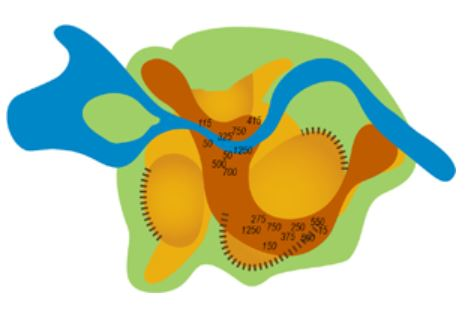
\includegraphics[width=0.50\textwidth]{billeder/Byudviklingsprincipper4}
\caption{Figuren viser det område hvor Aalborg skal udvikle sig på, i følge kommuneplanen.}
\label{fig:Byudviklingsprincipper4}
\end{figure}


Det er vigtigt, at Aalborg i fremtiden udvikler sig til at blive en blå by (en by med mange søer og vandløb). Der skal etableres en blå ring rundt om byen, bestående af en række søer og vandløb, ikke kun pga. rekreative årsager, men også funktionelle årsager, da søerne og vandløbene kan aflede en del af de vandmasser, som vil komme i fremtiden. Søerne skal etableres i tidligere råstofgrave, som ligger rundt om Aalborg. Figur \ref{fig:Byudviklingsprincipper5} viser Aalborg som en blå by.

\begin{figure}[H] 
\centering
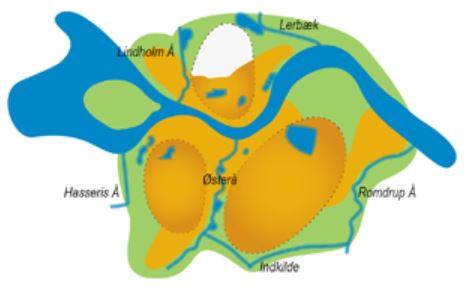
\includegraphics[width=0.50\textwidth]{billeder/Byudviklingsprincipper5}
\caption{Figuren viser Aalborg Kommunes vision af Aalborg som en blå by}
\label{fig:Byudviklingsprincipper5}
\end{figure}

Aalborg skal ikke kun være en blå by, det skal også være en grøn by. Der skal etableres en grøn ring rundt om byen og på bakkerne, langs fjorden og i Østerådalen skal der laves en række grønne forbindelser. Aalborgs markante bakketoppe skal i fremtiden fremstå som skovklædte kendetegn. Figur \ref{fig:Byudviklingsprincipper6} viser Aalborg Kommunes vision af Aalborg som en grøn by.

\begin{figure}[H] 
\centering
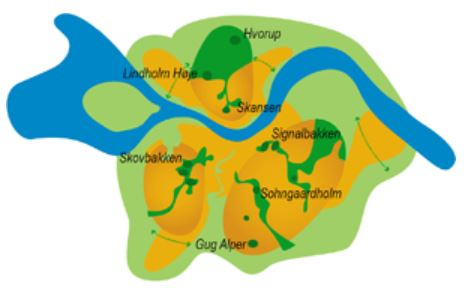
\includegraphics[width=0.50\textwidth]{billeder/Byudviklingsprincipper6}
\caption{Figuren viser Aalborg Kommunes vision af Aalborg som en grøn by}
\label{fig:Byudviklingsprincipper6}
\end{figure}


\subsection{Fokus på bykvalitet}
I Aalborg skal der være stort fokus på god bykvalitet, som er afhængig af stedet. Det er vigtigt, at velfungerende bygninger og byrum udvikles på baggrund af stedets særlige kvaliteter og potentialer, byens rum skal udvikles til at blive attraktive og rare at opholde sig i. Konkrete mål for bykvalitet er forskelligt fra nærmiljø til nærmiljø. Arkitektonisk kvalitet og kulturhisotrie skaber en identitet til nærmiljøerne og dette skal sikres. Byens kvaliteter skal være forskellige så der er noget for både beboere, studerende, kunder, turister og arbejdere.

\begin{figure}[H] 
\centering
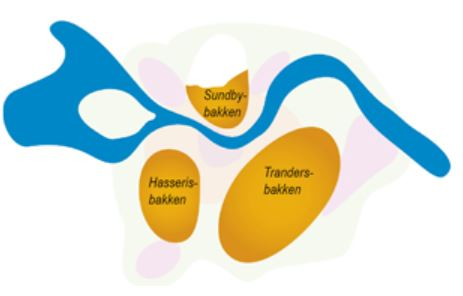
\includegraphics[width=0.50\textwidth]{billeder/Bykvalitet1}
\caption{Figuren viser Aalborgs tre store bakkeområder, Hasseri-, Sundby- og Trandersbakken.}
\label{fig:Bykvalitet1}
\end{figure}

Aalborg er en bakkeby og dette skal tydeligt kunne ses på byen. Landskab, udsigt, lys og luft er nogle særlige kvaliteter, som skal fremmes ved Aalborgs tre store bakker. På Figur \ref{fig:Bykvalitet1} ses Aalborgs tre store bakkeområder. Det er vigtigt, at bebyggelsen giver plads til naturen. Aalborgs forskellige forstadsområder skal udvikles, som veldefinerede nærmiljøer med lokal identitet og særpræg. Udviklingen af forstadsområderne skal blandt andet ske ved at oprette en række gode mødesteder, en forbedret infrastruktur, nye boligformer og ved nye multifunktionelle bygninger og byrum, som skal skabe liv. Fremtidige forstadsområder skal udvikles mere bæredygtigt, blandt andet ved at gå væk fra enfamiliehuse, da dette vil åbne op for større naturområder og mindre behov for biler.

\begin{figure}[H] 
\centering
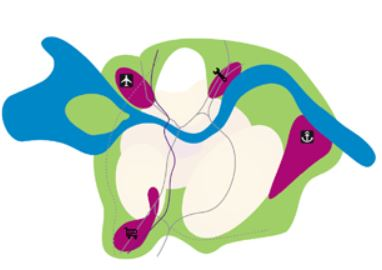
\includegraphics[width=0.50\textwidth]{billeder/Bykvalitet2}
\caption{På figuren er Aalborgs primærer erhversområder markeret med lilla.}
\label{fig:Bykvalitet2}
\end{figure}

Aalborg skal i fremtiden have fire veldefinerede erhvervsområder, lufthavnsområdet, City Syd, Aalborg Havn og Nørre Uttrup, områderne kan ses på Figur \ref{fig:Bykvalitet2}. De fire erhvervsområder skal have en høj funktionalitet, de skal være nemt tilgængelige og der skal være gode muligheder for transport af varer til og fra dem. City Syd skal i fremtiden være karakteriseret af storskalashopping. Området skal derved fungere, som et supplement til midtbyen. Aalborg Havn og lufthavnsområdet skal sikres fremtidige udviklingsmuligheder. 

\subsection{Nødvendige forbindelser - mobilitet}
I fremtiden skal en væsentlig større del af trafikken i Aalborg foregå med bæredygtige transportformer. I bymidten skal fodgængere, cyklister og kollektiv trafik prioriteres over biler. Et cykelstinet af høj kvalitet skal sikre cyklisterne meget høj tilgængelighed i Aalborg. Det skal være nemt og enkelt at tage fra midtbyen til universitetet, universitetshospitalet, Østhavnen og lufthavnen. Nye parkeringspladser i midtbyen skal begrænses, og i stedet opføres i store P-huse eller P-kældre langs randgaderne. På Figur \ref{fig:Mobilitet1} ses de veje, som primært skal aflaste trafikken i vækstakse området.

\begin{figure}[H] 
\centering
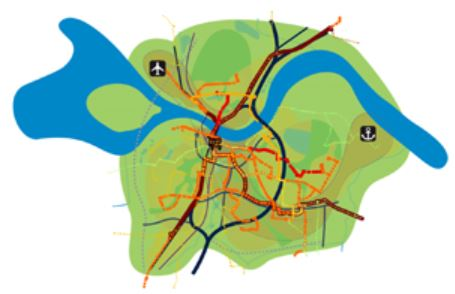
\includegraphics[width=0.50\textwidth]{billeder/Mobilitet1}
\caption{Figuren viser de veje der primært skal aflaste trafikken i vækstakse området.}
\label{fig:Mobilitet1}
\end{figure}

\subsection{Opsamlende analyse}
Aalborgs Kommunes kommuneplan ligger stort fokus på, at Aalborg skal udvikle sig bæredygtigt både for miljøet og for menneskerne i byen. Kommuneplanen ligger stort fokus på bæredygtigt transport, hvor de vil have bilerne ud af centrum og i stedet for have busser, cyklister, fodgængere og en letbane ind i centrum. Letbanen bliver ikke til noget, da det ikke var muligt at få statslig støtte til projektet, hvilket er et stort tilbageslag for Aalborg Kommunes vision for Aalborg, da letbanen skulle bidrage markant til den bæredygtige transport. I stedet for en letbane har kommunen etableret en del af en busvej, som efter planen skal starte ved Aalborg Busterminal og slutte ved Aalborg Universitet og med en fremtidig endestation ved nybyggeriet Aalborgs Universitetshospital. Busvejen skal gå igennem Øgadekvarteret, Vejgaard, under motorvejen og forbi Gigantium. Aalborg Kommunes plan om at få borgerne til at droppe bilerne til fordel for offentlig transport, bliver svært da det ofte kan føre til længere transport tider og nogle gange også være dyrere. Andre grunde til at det kan være svært for kommunen at få folk til at skifte fra bil til offentlig transport er f.eks. kultur, vaner og frihedsfølelsen ved at køre en bil man ejer. Mange vælger offentlig transport fra, men nogle vælger cyklen til. En af grundene til dette kan være Aalborg Kommunes store fokus på at lave et godt cykelstinet. Aalborg Kommune vil have en fortætning af byen omkring en række knudepunkter, se Figur \ref{fig:Vaekstakse3}, langs vækstaksen. Ved disse knudepunkter vil kommunen have en høj mobilitet med mulighed for at skifte mellem diverse transportformer, dette kan være et problem da en fortætning af byen, kan give mangel på plads til f.eks. parkeringspladser. En løsning på dette vil være etablering af en række P-kældere, hvilket igen bliver et problem, da disse er relativt dyre. Kommunens plan om at adskille by og tunge erhversområder er meget godt for bymilljøet og erhvervet. Det er godt for erhvervsområderne på den måde, at det markant nedsætter transporttiden, da lasten ikke skal igennem byen først, men derimod bare kan transporteres direkte videre med skib og lastbil. Det gode for bymiljøet er, at der kommer færre lastbiler igennem byen, som både forurener meget og forsinker trafikken. Kommunens plan om et etablere en tredje Limfjordsforbindelse og en paralleltunnel er i følge en VVM-undersøgelse en meget god samfundsinvestering som vil spare samfundet for en stor mængde rejsetimer og penge.

Aalborg Kommune er en kommune, som i lang tid har haft fokus på bæredygtighed, hvilket blandt andet kan ses på Aalborgs Bæredygtighedsfestival. Dette kan også ses i Aalborgs Kommunes kommuneplan, hvor der bliver lagt fokus på, at Aalborg skal være en blå og grøn storby, hvor der blandt andet skal være en række søer, vandløb og grønne områder i og omkring Aalborg. Det er ikke tilfældigt at Aalborg Kommune ligger stort fokus på at udvikle kommunen bæredygtigt. Nogle af grundene hertil er, at det er "in" at være og tænke bæredygtigt, mange borgere går op i bæredygtighed også ligger der en masse lovgivning til grund for dette, blandt andet planloven, som blandt andet kræver at kommunerne udarbejder strategiredegørelser for blandt andet "mindskelse af miljøbelastning" og "fremme af en bæredygtig byudvikling og byomdannelse", dette kaldes også "Agenda 21". Søerne der skal laves omkring Aalborg er ikke kun til rekreativt brug. Et eksempel på en af søerne som ikke skal bruges rekreativt er, søen som er blevet dannet i Aalborg Portlands kridtgrav, den skal bruges til at køle det kommende supersygehus. Etablering af diverse nye vandløb, søer og grønne området inde i centrum af Aalborg, kan give problemer, da kommunen på samme tid vil have at der sker en fortætning af byen. Pladsmangel vil højst sandsynligt føre til at, færre søer, vandløb og grønne områder bliver etableret i centrum. 

I kommuneplanen fremgår det at de tre store bakkeområdet Hasseri-, Sundby- og Trandersbakken, skal være præget af landskab, udsigt, lys og luft, hvilket betyder at der skal være grønne og åbne områder på bakkerne. Et andet sted i kommuneplanen står der at fremtidig byudvikling og byfortætning primært skal ske i disse områder, grundet stigende vandstande i fremtiden. For at dette kan lade sig gøre vil kommunen have at områder skal bestå af nye boligformer og gå væk fra de traditionelle enfamiliehuse.



\section{Lokalplan - Strøybergs Palæ}
En lokalplan bruges til at fastlægge bestemmelser for udviklingen af et område, som i dette tilfælde er Strøybergs Palæ. Lokalplanen skal være med til at give et overblik over området, samt være en plan over for hvordan området skal bruges og hvad der skal overholdes. Med en lokalplan sikrer man, at alle er enige om områdets udvikling og at bevaringsværdige bygninger bliver bevaret efter planloven. 

\begin{figure}[H] 
\centering
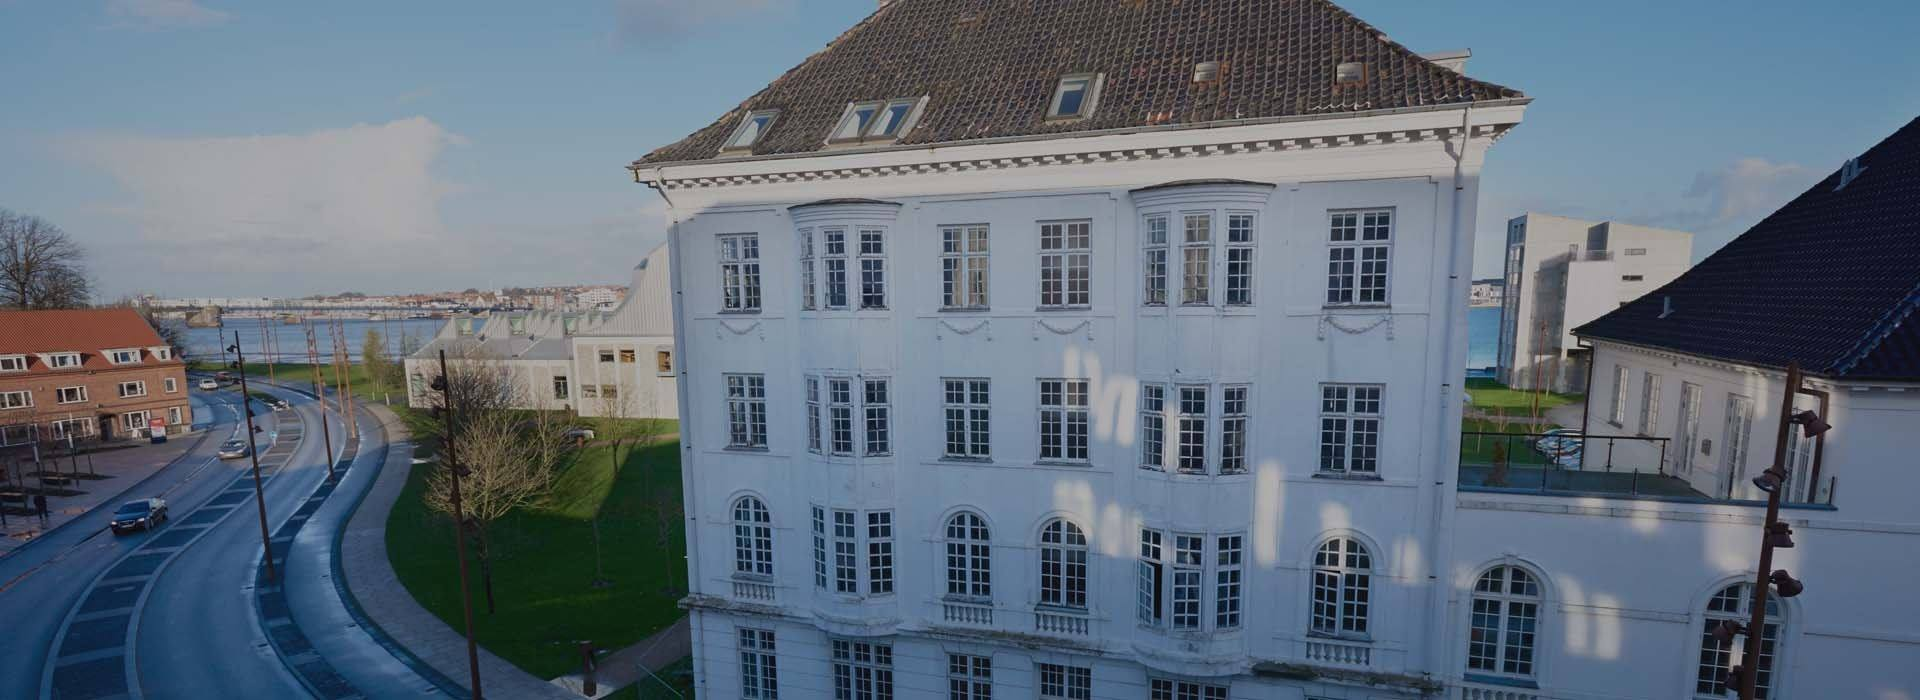
\includegraphics[width=0.50\textwidth]{billeder/Lokalplan3}
\caption{Strøybergs Palæ}
\label{fig:Lokalplan3}
\end{figure}



Den 12. november 2012 blev en ny lokalplan for Strøybergs Palæ vedtaget af Aalborg byråd (1-1-107 Strøybergs Palæ). I lokalplanen blev der fremlagt et forslag om at lave en tilbygning til hovedbygningen. Tilbygningen til Strøybergs Palæ skal bygges inden for lokalplanens fastlagte rammer. I dette afsnit gennemgås lokalplanen for Strøybergs Palæ, efter hvad der har relevans for opførelsen af en tilbygning. 

\begin{figure}[H] 
\centering
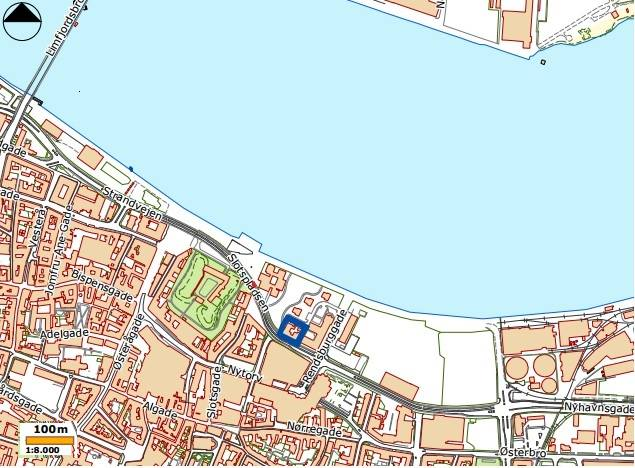
\includegraphics[width=0.50\textwidth]{billeder/Lokalplan1}
\caption{Kort over Aalborg Havnefront med Strøyberg Palæs lokalplanområde markeret med blåt}
\label{fig:Lokalplan1}
\end{figure}

Lokalplanen udgør et område, med et areal på 1200$ m^{2} $. Området ligger i tilknytning til havnefronten, ca. 100m fra Limfjorden, se Figur \ref{fig:Lokalplan1} . Strøybergs Palæ anvendes primært som en kontorbygning. Området er delt op i to dele, delområde A og B, se Figur \ref{fig:Lokalplan2}. Delområde A er den bevaringsværdige hovedbygning og delområde B er den bevaringsværdige sidebygning. Begge delområderne er kategoriseret til at have en bevaringsværdi på middel. Dvs. ved eventuel ombygning af bygningerne, skal der tages hensyn til det oprindelige udseende af bygningen. Tilbygninger og nybyggeri skal tilpasses det bevaringsværdige, men må stadig gerne udtrykke noget nutidigt design.



\begin{figure}[H] 
\centering
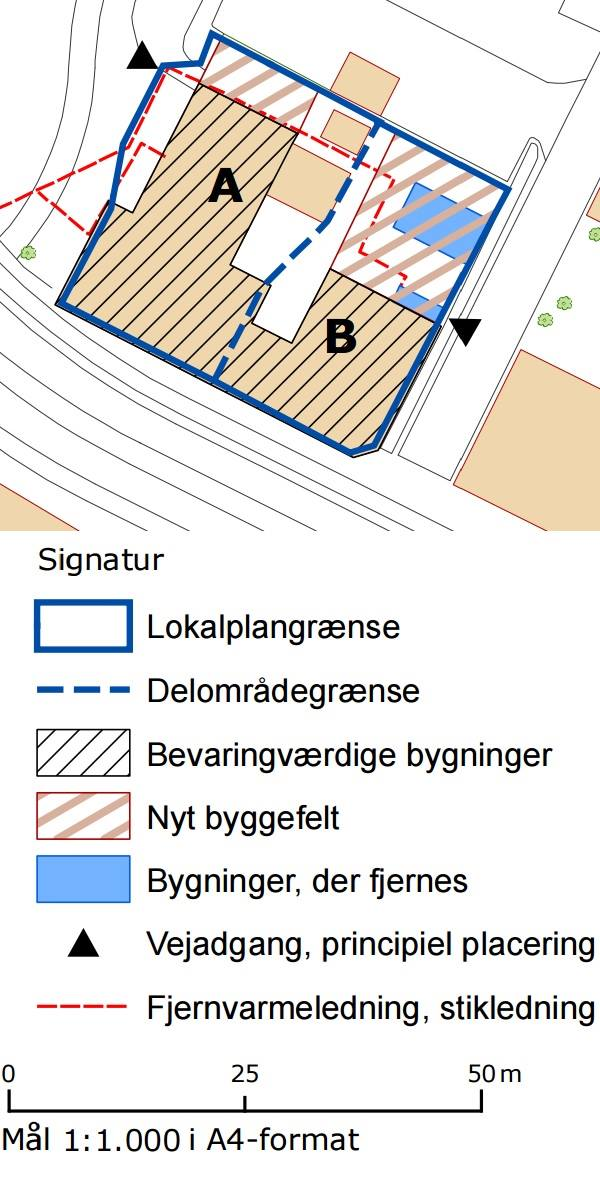
\includegraphics[width=0.50\textwidth]{billeder/Lokalplan2}
\caption{På denne figur ses delområde A og B, samt byggefeltet inden for lokalplanområdet, hvor tilbygningen kan være}
\label{fig:Lokalplan2}
\end{figure}

I Lokalplanen har man opstillet restriktioner for tilbygningen. Nedenfor vil de mest hovedsagelige blive gennemgået.

Tilbygningen skal bygges inden for byggefeltet illustreret på Figur \ref{fig:Lokalplan2}. Dette kræver, at mindre bygninger på området, som ikke er bevaringsværdige, nedrives til fordel for tilbygningen. Der er fastlagt for det samlede byggeareal i delområde A, at der maksimalt må være en bebyggelsesprocent på 350 procent. For delområde B er bebyggelsesprocenten maks. 320 procent. 

Strøybergs Palæ, som bygningen står nu, er op til 4½ etager og har en højde på ca. 22 meter. Dvs. 3 etager, 1 kælder og en tagetage. For den nye bebyggelse kan der bygges samme antal etager samt en tagetage, dog må den maksimale højde ikke overskride 19 meter. Med denne højde menes det ikke at have nogen effekt på udsigten til kysten, idet der er opført tre punkthuse med op til 7 etager, mellem lokalplanområdet og Limfjorden. Der kan være mulighed for at bygge kælderarealer til parkering, depot, teknik og lignende. Hvis der vælges at bygge en kælderetage, må der maksimalt være en lofthøjde på 2 meter over terræn ved område B, og 1.25 meter for område A. På grund af fremtidige vandstandsstigninger, skal kælderetagen desuden sikres mod oversvømmelse eller blot tåle at blive oversvømmet. 

Der ud over sættes der i høj grad krav til det arkitektoniske ved tilbygningen. Der er ikke specifikke krav til udformningen af tilbygningen, dog er det vigtigt, at tilbygningen har samme stil, som det eksisterende. Facaderne på tilbygningen skal være ensartede mure og der må kun benyttes lyse farver af hvide nuancer. Ved sadeltag, må der kun være sortglaserede vingetegl. Hvis tilbygningen skal være i forlængelse af de eksisterende, så skal overganges markeres i form af eksempelvis materialeskift i et bånd.  Som tidligere nævnt, vil det være fordelagtigt hvis bygningen samtidig udviser noget nutidigt design, men uden at skille sig ud. 

Ved ombygning og nybyggeri, opstår et krav fra Miljøministeriet om støjisolation. Den vejledende grænseværdi for trafikstøj, som er fastlagt af Miljøministeriet, skal overholdes. Støjisolation bliver nødvendigt for lokalplanområdet, idet det ligger ud til Nyhavnsgade, som har en trafikbelastning på 10.850 biler i årsdøgntrafik taget i en måling i 2011. Støjbelastningen indendørs skal bringes under $ L_{den} $ 38 dB for kontorbygninger eller lignende, og da man vil undgå at ændre på bygningens ydre design, skal isoleringen foretages på indersiden. For udendørsarealer må støjniveauet ikke overstige $ L_{den} $ 58 Tilbygningen må ikke tages i brug før det er dokumenteret at bygningen overholder grænseværdien for støj.


%\chapter{Interessentanalyse}
I dette afsnit vil de interessenter, som har en betydning for tilbygningen af Strøybergs Palæ analyseres gennem fire typeområder; identificering-, prioritering-, kortlægning- og konklusion af interessenter. Interessentanalysen skal have til formål at få styr på hvem der har interesse i projektet, samt opnå forståelse for grundlaget for opførelsen af projektet.
Interessenter er alle som på den ene eller anden måde bliver påvirket af det pågældende projekt. Dette kan omfatte personer, grupper, organisationer, virksomheder mm. Derudover kan det også udvides til ”ikke-talende” interessenter som eksempelvis miljøet. Da der er mange interessenter, som man kan tage højde for, er der valgt at tage udgangspunkt i følgende interessenter:

\begin{itemize}
\item Bygherren/ejeren
\item Investorer
\item Kommunen
\item Forbrugere
\item Rådgivere
\end{itemize}

I det følgende vil disse interessenter analyseres ud fra overnævnte typeområder.

\section{Analyse}

\begin{figure}[H] 
\centering
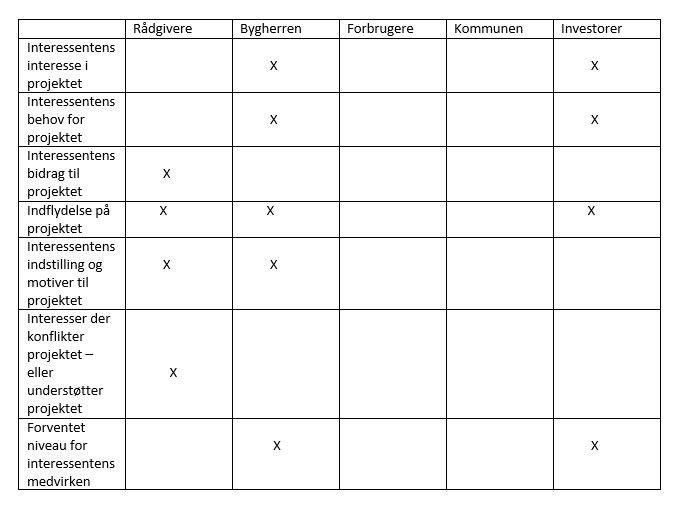
\includegraphics[width=0.80\textwidth]{billeder/IA1}
\caption{Tabel der viser de forskellige intersenters relevans for projektet.}
\label{fig:IA1}
\end{figure}

\subsection{Indflydelse}

\begin{itemize}
\item Bygherren/ejeren
\item Investorer og rådgivere
\item Kommunen
\item Forbrugere
\end{itemize}

Ved indflydelse menes der hvor relevant interessentens indflydelse er i forberedelsesarbejdet for et. Rækkefølgen er sat fra et til fire, hvor et har størst relevans. I dette tilfælde, er det i forhold til bygningsprojektet ved Strøybergs palæ.

I dette afsnit vil listen blive argumenteret for.

Ethvert byggeprojekt har en ejer, som i oftest tilfælde også er bygherren, altså en person eller organisation med et ønske om at opføre en konstruktion. Disse har sandsynligvis en lang række kriterier for projektet og vil gerne diktere retningen, som projektet skal tage. Desuden kan ejeren som regel nedlægge projektet til enhver tid, så længe alle er blevet betalt for det arbejde de måtte have udført. 

Hernæst er eventuelle investorer i projektet også yderst indflydelsesrige, idet projektet muligvis ikke er muligt at gennemføre uden deres økonomiske støtte til projektet. Investorerne kan altså også i og for sig nedlægge projektet, hvis det eventuelt ikke tager deres ønskede retning, ved at trække deres økonomiske støtte.

Desuden er rådgivere, ingeniører, arkitekter og økonomer også væsentlige brikker i den samlede forberedelsesfase. Uden deres hjælp ville alle større projekter ikke kunne gennemføres, idet der enten ville mangle beregninger, designs eller orden i økonomien.

Foruden ejeren og eventuelle investorer, spiller kommunen, hvori projektet skal gennemføres, også en stor rolle, eftersom den har dikteret en lokalplan, som skal følges, dog med mulighed for kompensation. Kommunen sætter med lokalplanen altså rammerne for projektet, hvormed de har den afgørende indflydelse i planlægningsfasen. Herefter er det usandsynligt, at kommunen har stor indflydelse, med mindre der bliver bygget uden for lokalplanens rammer. I sådan et tilfælde skal kommunen vurdere om der skal laves om eller om det er tilladt.
 
Forbrugerne har tilnærmelsesvis ingen indflydelse på projektet, idet de ikke ejer noget eller bidrager økonomisk til projektet.

\subsection{Medvirken}
Ved medvirken menes, hvor vigtig interessentens aktive medvirken er, i forhold gennemførelsen af projektet. Prioriteringen af interessenterne er valgt som følgende:

\begin{itemize}
\item Bygherren/ejeren
\item Investorer
\item Forbrugere og kommunen
\end{itemize}

Nedenfor vil denne prioritering argumenteres
Som højeste prioritet er det vurderet, at bygherren har den største medvirken til projektet. Grundlaget for, at projektet om tilbygningen til Strøybergs Palæ kan fuldføres, er først og fremmest, at der er et firma eller en privat person, som betaler for udførelsen af projektet. Bygherren er også den, som skal opføre projektet, efter de funktions- og designkrav, hvis der er en eventuel køber af slutproduktet. Det er derfor vigtigt, at bygherren er vel-informeret under hele projektet, da bygherren i første omgang ejer projektet. 

Bygherren har altså den største medvirken til projektet i den forstand, at uden en bygherre, ville projektet aldrig kunne realiseres. 

Herefter vurderes det, at investorerne har næsthøjeste prioritet i forhold til medvirken. Investorerne kan siges at være på sidekanten af projektet. De stiller ingen konkret arbejdsindsats til rådighed, men kan dog komme med mindre indvirkninger i mindre dele af projektet. Det er vigtigt, at de er involveret i hele projektet, da det er dem som skal investere i slutproduktet. 

Til sidst er der de eksterne interessenter, forbrugere og kommunen. Forbrugernes medvirken er ikke nødvendigt til opførelsen af projektet, men er interesseret i slutproduktet.  Kommunen har ikke nogen reel medvirken i projektet, men er interesseret i projektet som helhed, da det er en del af Aalborgs udvikling. Som nævnt i kapitel XX angående kommuneplanen, så er Aalborg på vej mod at være en kompetence by, hvilket betyder, at der vil være et større behov for kontorbygninger og boliger. Kommunen ser derfor positivt over for projekter som dette.

\section{Analyse opsamling}
Ser man på listerne, for henholdsvis indflydelse og medvirken, er de ens. Herved kan de konkluderes, at det øverste navn på listen har den afgørende stemme. Disse personer eller organisationer er hvad man kalder ressourcepersoner. Dette betyder samtidig, at beslutningen om ikke at gennemføre en tilbygning, som de tidligere ejere, TWT Aalborg, havde tænkt sig at gennemføre højst sandsynligt kom fra ejeren/bygherren. Eftersom det ikke har været muligt at skaffe informationer herom, er det kun muligt at spekulere i hvorfor de nuværende ejere, Calum A/S, ikke har valgt at gennemføre projektet. 

Den mest sandsynlige årsag ville være vedrørende økonomi. Måske har projektet vist sig at være for dyrt til at kunne betale sig. Herudover kunne det skyldes hensyntagen til naboer, hvis udsigt muligvis kunne blive blokeret af en eventuel fleretagesbygning. 

Om end usandsynligt, så er det muligt, at Calum A/S blot har anset tilbygningen for værende unødvendig.


%\chapter{Delkonklusion}
Dette afsnit er ikke færdigt endnu.

%\chapter{Problemanalyse}
Projektet er baseret på et ønske om at opføre en tilbygning til Strøybergs Palæ, for på den måde at udvide lejligheds antallet. Tilbygningen skal opføres i henhold til Aalborg Kommunes kommuneplan og lokalplanen der er gældende for området. Funderingsmetoden skal bestemmes ud fra en analyse af jordbundsforholdene i området.

 
NB: dette er stadig work in progress.


\section{Problemformulering}
I dette projekt vil det følgende problem blive belyst:

\textit{Hvordan kan et fundament og et stålskelet til en tilbygning til Strøybergs Palæ dimensioneres ud fra en jordbundsundersøgelse samt et trækforsøg af en stålstang.}

\section{Problemafgrænsning}
I projektet vil vi afgrænse os fra følgende emner:

\begin{itemize}
\item Prisvurdering af tilbygningen.
\item Tilbygningens indeklima og energ.
\item Tilbygningens miljøbelastning og materialernes miljøpåvirkning.
\item Tilbygningens Ulykkeslaster og brandsikring.
\item Vej og trafik.
\end{itemize}


\chapter{Laster}
I det følgende afsnit vil de laster der påvirker tilbygningen til Strøybergs Palæ. Lasterne der påvirker konstruktionen er nytte-, egen-, vind- og snelast. Lasterne skal være kendt, før bygningen og fundamentet kan dimensioneres.

\section{Nyttelast}
Nyttelast er en last der ikke virker permanent på en bygning, men derimod er varierende og kommer af anvendelse af en bygning. Nyttelast er den last som mennesker og inventar påvirker en konstruktion med. Nyttelast dækker over to laster, den transiente del (laster der varer over en til tre dage) og den vedvarende del (laster der varer over fem til ti år).

Nyttelast regnes på to forskellige måder, en jævnt fordelt fladelast $ q_{k} $ målt i $ \SI{}{kN/m^2} $ og en punktlast $ Q_{k} $, målt i kN. Disse to nyttelaster kan ikke optræde samtidigt. Fladelasten bruges til en global eftervisning af bæreevne og punktlasten bruges til en lokaleftervisning af bæreevne.


Nyttelasten, der virker på tilbygningen, er ens på alle etager. Bygningen er beregnet til boliger og går derfor ind under kategori A, som beskrevet i den tilhørende Eurocode. I kategori A regnes der med en anbefalet karakteristisk jævnt fordelt nyttelast på $\SI{2}{kN/m^2}$ og en punktlast på $\SI{2}{kN/m^2}$


\newpage

\section{Egenlast}
	Egenlasten er udregnet ud fra 3D modeller, så materialeforbruget fremgår klart og tydeligt. Egenlasten indebærer ydervæggene, etageadskillelse, taget og naturligvis stålskelettet.
	
	Eftersom der regnes på en ramme ved siden af midten af hele bygningen, ser rammen således ud
\begin{figure}[H] 
	\centering
	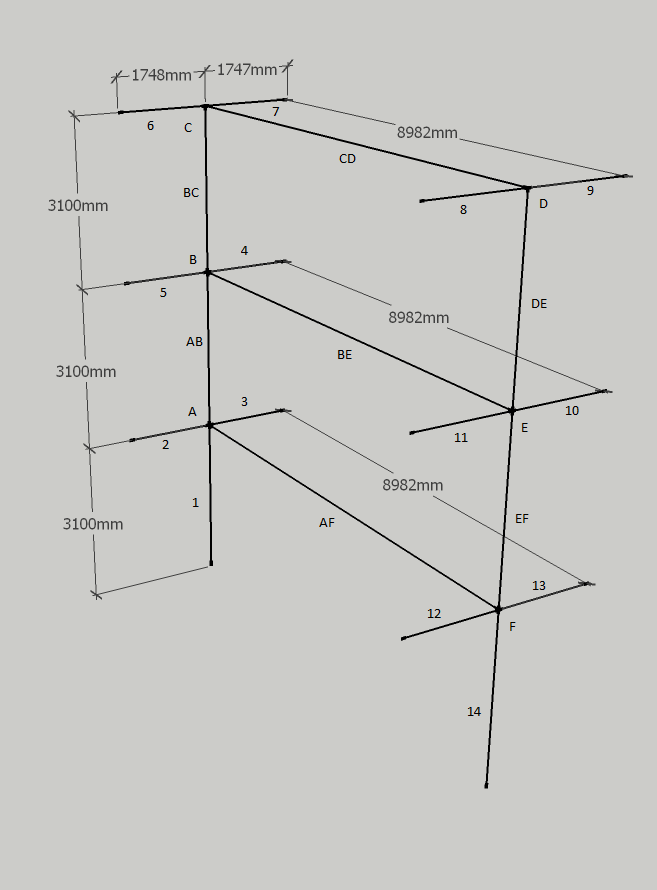
\includegraphics[width=0.7\textwidth]{billeder/Staaldimensioner_5}
	\caption{Viser en 3D model af rammens stållayout }
	\label{fig:EL1}
\end{figure}	
	\newpage
	Denne ramme bærer altså denne mængde af bygningen
\begin{figure}[H] 
	\centering
	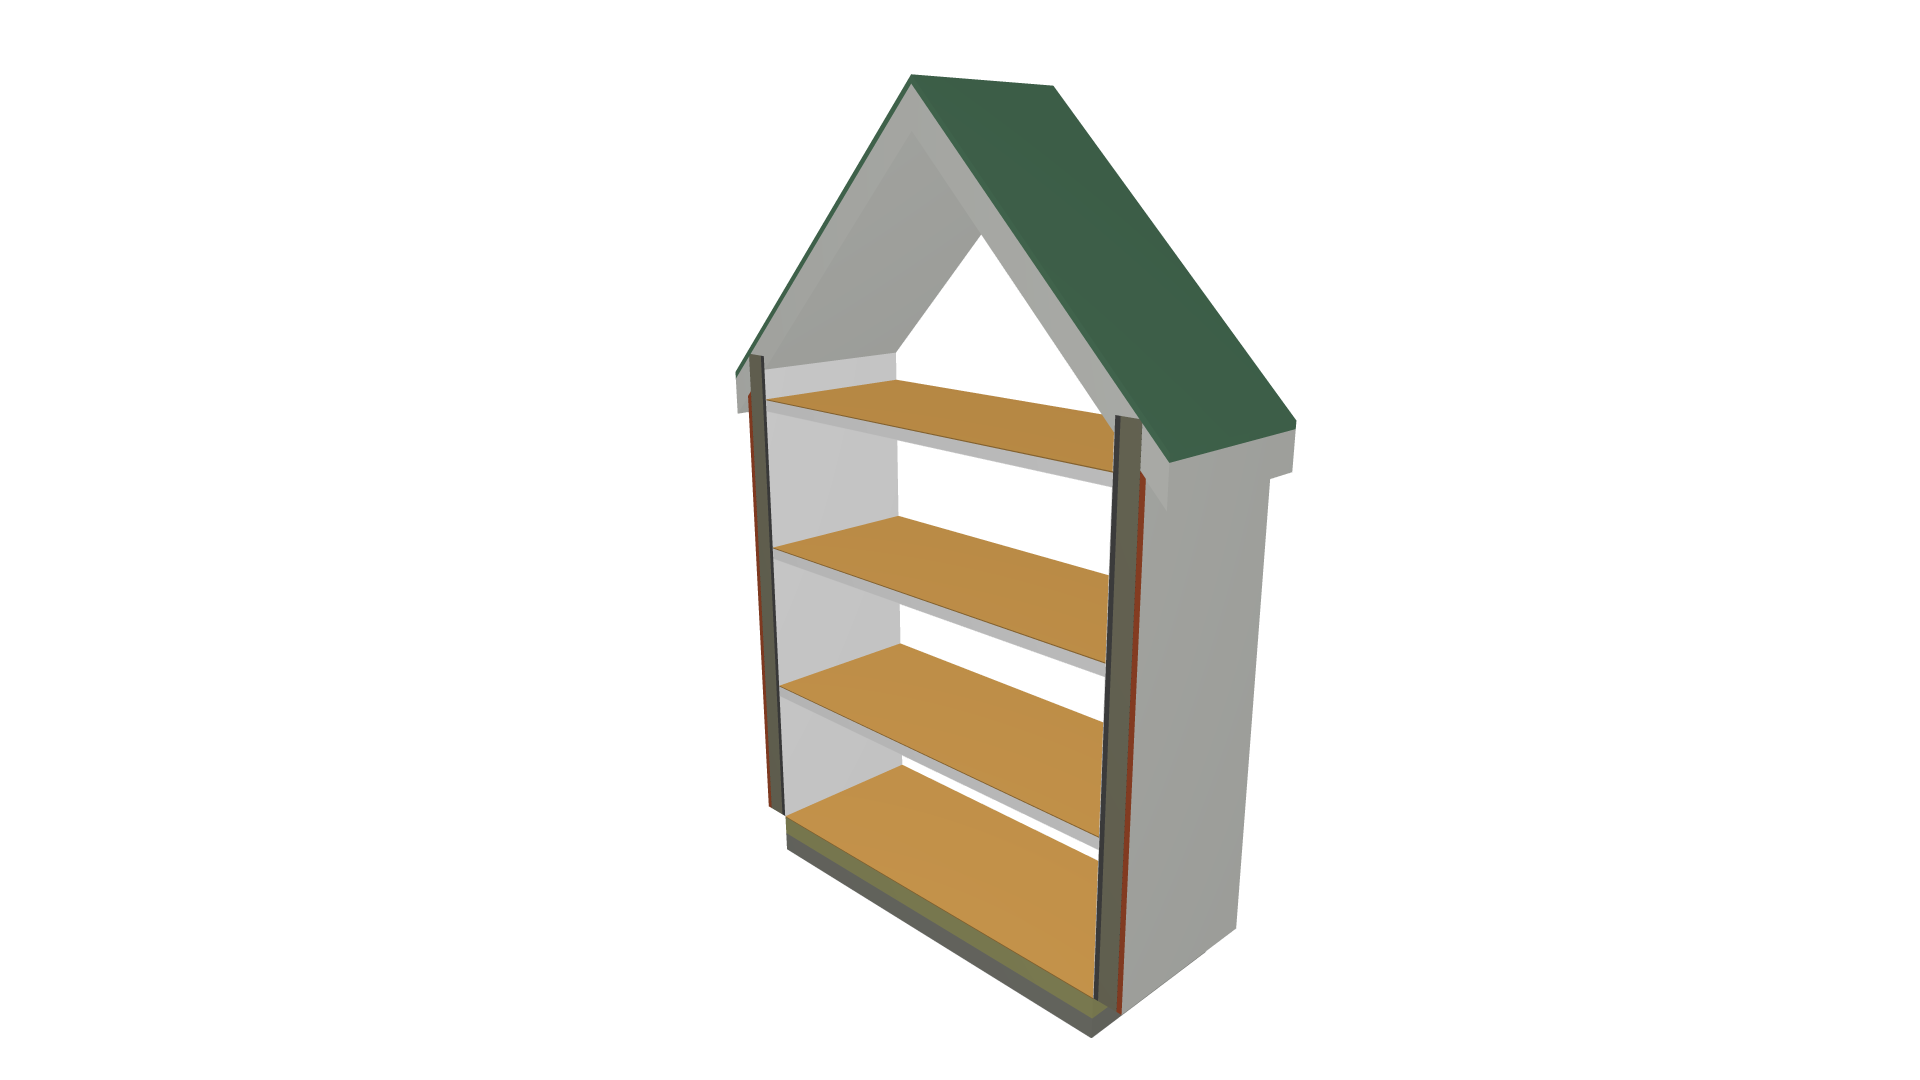
\includegraphics[width=1\textwidth]{billeder/Tvaersnit1}
	\caption{Viser en 3D model af de elementer, som stålrammen på Figur \ref{fig:EL1} bærer}
	\label{fig:EL2}
\end{figure}

I tabellen herunder ses ydervæggenes opbygning. Tallene er for den ene side af bygningen, altså det som halvdelen af rammen bærer.
\begin{table}[H]
	\centering
	\begin{tabular}{lll|l|ll|l|l}
		\cline{4-4} \cline{7-7}
		&                                                        &      & Mængde ($m^{3}$) &                             &      & Vægt (kg) &                             \\ \hline
		\multicolumn{1}{|l|}{}           & \multicolumn{1}{l|}{Densitet ($\dfrac{kg}{m^{3}}$)} & St.  & 1. sal                       & \multicolumn{1}{l|}{2. sal} & St.  & 1. sal    & \multicolumn{1}{l|}{2. sal} \\ \hline
		\multicolumn{1}{|l|}{Teglsten}   & \multicolumn{1}{l|}{1500}                              & 1,17 & 1,17                         & \multicolumn{1}{l|}{1,17}   & 1755 & 1755      & \multicolumn{1}{l|}{1755}   \\ \hline
		\multicolumn{1}{|l|}{Mineraluld} & \multicolumn{1}{l|}{115}                               & 4,33 & 4,33                         & \multicolumn{1}{l|}{4,33}   & 498  & 498       & \multicolumn{1}{l|}{498}    \\ \hline
		\multicolumn{1}{|l|}{Gips}       & \multicolumn{1}{l|}{900}                               & 0,13 & 0,13                         & \multicolumn{1}{l|}{0,13}   & 117  & 117       & \multicolumn{1}{l|}{117}    \\ \hline
		\multicolumn{1}{|l|}{SUM}        & \multicolumn{1}{l|}{}                                  & 5,63 & 5,63                         & \multicolumn{1}{l|}{5,63}   & 2371 & 2371      & \multicolumn{1}{l|}{2371}   \\ \hline
	\end{tabular}
	\caption{Viser densitet af de anvendte materialer, samt materialeforbruget og massen på de forskellige etager}
	\label{tabel:EL1}
\end{table}

I tabellen herunder ses gulvenes opbygning. Tallene er for den ene side af bygning, altså det som halvdelen af rammen bærer.
\begin{table}[H]
	\centering
	\begin{tabular}{lll|l|ll|l|l}
		\cline{4-4} \cline{7-7}
		&                                                        &       & Mængder ($ m^{3} $) &                            &      & Vægt (kg) &                             \\ \hline
		\multicolumn{1}{|l|}{}          & \multicolumn{1}{l|}{Densitet ($ \dfrac{kg}{m^{3}} $)} & St.   & 1. sal                        & \multicolumn{1}{l|}{2.sal} & St.  & 1. sal    & \multicolumn{1}{l|}{2. sal} \\ \hline
		\multicolumn{1}{|l|}{Træ}       & \multicolumn{1}{l|}{500}                               & 0,314 & 0,314                         & \multicolumn{1}{l|}{0,314} & 157  & 157       & \multicolumn{1}{l|}{157}    \\ \hline
		\multicolumn{1}{|l|}{Hul beton} & \multicolumn{1}{l|}{2000}                              & 3,45  & 3,45                          & \multicolumn{1}{l|}{3,45}  & 6906 & 6906      & \multicolumn{1}{l|}{6906}   \\ \hline
		\multicolumn{1}{|l|}{Gips}      & \multicolumn{1}{l|}{900}                               & 0,157 & 0,157                         & \multicolumn{1}{l|}{0,157} & 141  & 141       & \multicolumn{1}{l|}{141}    \\ \hline
		\multicolumn{1}{|l|}{SUM}       & \multicolumn{1}{l|}{}                                  & 3,92  & 3,92                          & \multicolumn{1}{l|}{3,92}  & 7204 & 7204      & \multicolumn{1}{l|}{7204}   \\ \hline
	\end{tabular}
	\caption{Viser densitet af de anvedte materialer, samt materialeforbruget og massen på de forskellige etager}
	\label{tabel:EL2}
\end{table}

\newpage
I tabellen herunder ses tagets opbygning. Tallene er for den ene side af taget, altså det som halvdelen af rammen bærer.
\begin{table}[H]
	\centering
	\begin{tabular}{l|l|l|l|}
		\cline{2-4}
		& Densitet ($ \dfrac{kg}{m^{3}} $) & Mængde ($ m^{3} $) & Vægt (kg) \\ \hline
		\multicolumn{1}{|l|}{Tagsten}    & 2000                              & 0,522                        & 1044      \\ \hline
		\multicolumn{1}{|l|}{Mineraluld} & 115                               & 26,1                         & 3003      \\ \hline
		\multicolumn{1}{|l|}{SUM}        &                                   & 26,6                         & 4047      \\ \hline
	\end{tabular}
	\caption{Viser densitet af de anvedte materialer, samt materialeforbruget og massen af taget}
	\label{tabel:EL3}
\end{table}

Eftersom det i udregningen af egenlasten ikke vides, hvilke stålprofiler der skal benyttes, bliver disse indsat som konstanter i udregningerne, hvorved man efterfølgende i styrkeberegningerne kan finde frem til hvilke typer, der er passende.

\begin{figure}[H] 
	\centering
	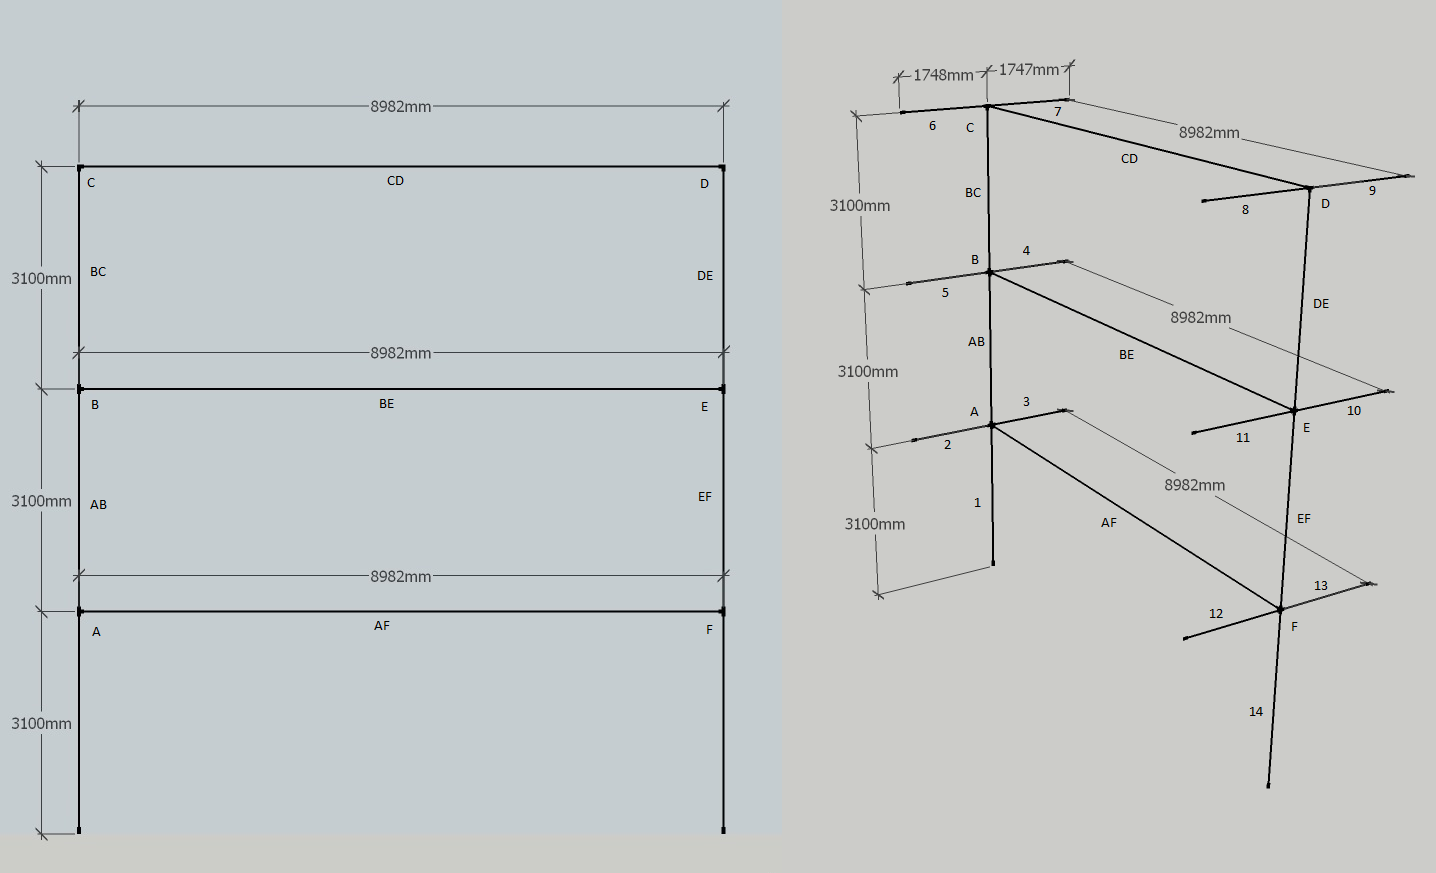
\includegraphics[width=1\textwidth]{billeder/Staaldimensioner_6}
	\caption{Viser en 3D model af stålrammen samt et tværsnitlayout}
	\label{fig:EL3}
\end{figure}

Beregnigner for egenlast i punkterne C og D. Konstruktionen er som nævnt symmetrisk omkring midten, så egenlasten bliver den samme i de to punkter. Denne tendens forsætter i de resterende punkter.
\newline
Tyngdeaccelerationen, g, sættes til $ 9,82\dfrac{N}{kg} $
\newline
Massen pr. meter for stålprofilerne betegnes, G, og måles i $ \dfrac{kg}{m} $. Størrelserne varierer og er ukendte. Så en stålbjælke eller søjle skrives eksempelvis som $ G_{CD} $.
\newline
Massen af taget, som den ene side af stålrammen bærer, angives som  $ m_{tag} $. Taget er ikke lavet af stål og kan derfor ikke ses på Figur \ref{fig:EL3}, men derimod på Figur \ref{fig:EL2}
\newline
Massen af gulvene, som den ene side af stålrammen bærer, angives som $ m_{gulv_{x}} $. Så et gulv der eksempelvis bæres af bjælken CD skrives $ m_{gulv_{CD}} $
\newline
\begin{center}
	$ P_{C/D}=m_{tag}\cdot g+G_{CD}\cdot g\cdot \dfrac{1}{2}\cdot 8,982m+m_{gulv_{CD}}\cdot g =110,5kN+k$
\end{center}

Beregninger for egenlast i punkterne B og E. 
\newline
Massen af murene angives som $ m_{mur_{x}} $. Så en mur der eksempelvis bæres af søjlen BC skrives $ m_{mur_{BC}} $.
\begin{center}
	$ P_{B/E}=P_{C/D}+G_{BE}\cdot g\cdot \dfrac{1}{2}\cdot 8,982m+m_{gulv_{BE}}\cdot g+m_{mur_{BC}}\cdot g+G_{BC}\cdot g\cdot 3,100m=204,5kN+k$
\end{center}

Beregninger for egenlast i punkterne A og F
\begin{center}
	$ P_{A/F}=P_{B/E}+G_{AF}\cdot g\cdot \dfrac{1}{2}\cdot 8,982m+m_{gulv_{AF}}\cdot g+m_{mur_{AB}}\cdot g+G_{AB}\cdot g\cdot 3,100m =298,5kN+k$
\end{center}

Beregninger for egenlasten i reaktionerne $ R_{1} $ og $ R_{2} $
\begin{center}
	$ P_{R_{1}/R_{2}}=P_{A/F}+m_{mur_{1/14}}\cdot g+G_{1}\cdot g\cdot \dfrac{1}{2}\cdot 3,100m=321,8kN+k$
\end{center}






\section{Vindlast}
Vindlast er den last som vind påvirker bygninger med og virker vinkelret på bygningers overflader. 

NOTE: evt. figur der viser hvordan vind virker på en konstruktion:

Følgende afsnit er beregnet ud fra Eurocode DS/EN-1991-1-4. Værdierne for diverse konstanter og variable er aflæst i det tilhørende danske nationale anneks.

I de følgende afsnit bliver basisvindhastigheden, ruhedesfaktoren, middelvindhastigheden, turbolensintensiteten, peakhastighedstrykket og vindtrykket på tilbygningen beregnet.








\subsection{Basisvindhastighed}
Basisvindhastigheden er afhængig af retningsfaktoren, årstidsfaktoren og grundværdien for basisvindhastigheden.

Følgende formel bruges til at beregne basisvindhastigheden:
\begin{align*}
v_{b} = c_{dir} \cdot c_{season} \cdot v_{b,0}
\end{align*}

Hvor:
\begin{itemize}
\item $v_{b}$ = basisvindhastigheden.
\item $v_{b,0}$ = grundværdien for basisvindhastigheden.
\item $ c_{season} $ = årstidsfaktoren.
\item $ c_{dir} $ = retningsfaktoren.
\end{itemize}
I dette tilfælde er $ v_{b,0} $ $ \SI{24}{m/s} $, $ c_{season} $ er 1,0, da bygningen står året rundt og $ c_{dir} $ sættes til 1,0, da dette er den anbefalede værdi.

\begin{align*}
v_{b} = 1,0 \cdot 1,0 \cdot \SI{24}{m/s}
\end{align*}

Dvs. basisvindhastigheden ved tilbygningen til Strøybergs Palæ er $ \SI{24}{m/s} $.








\subsection{Ruhedsfaktor}
Ruhedsfaktoren er afhængig af ruhedslængden, terrænfaktoren og bygningens højde over terræn.

Følgende formler bruges til at beregne ruhedsfaktoren
\begin{align*}
c_{r}(z) = k_{r} \cdot ln\left(\frac{z}{z_{0}}\right)
\end{align*}
\begin{align*}
k_{r} = 0,19 \cdot ln\left(\frac{z_{0}}{z_{0,II}}\right)^{0,07}
\end{align*}

Hvor:
\begin{itemize}
\item $ c_{r}(z) $ = ruhedsfaktoren i højden z.
\item $ k_{r} $ = terrænfaktoren.
\item z = bygningens højde over terræn.
\item $ z_{0} $ = ruhedslængden.
\item $ z_{0,II} $ =0,05m, som aflæst i Tabel XX
\end{itemize}

I dette tilfælde er z = 14.85 m, $ z_{0} $ er 0,3 m, grundet terrænkategori III er valgt.


Terrænfaktoren beregnes:
\begin{align*}
k_{r} = 0,19 \cdot ln\left(\frac{\SI{0,3}{m}}{\SI{0,05}{m}}\right)^{0,07} = 0,22
\end{align*}

Ruhedsfaktoren beregnes:
\begin{align*}
c_{r}(z) = 0,22 \cdot ln\left(\frac{\SI{14.85}{m}}{\SI{0,3}{m}}\right) = 0,86
\end{align*}

Dvs. ruhedsfaktoren i højden z ved tilbygningen ved Strøybergs Palæ er 0,86.







\subsection{Middelvindhastighed}
Middelvinhastigheden er afhængig af orografifaktoren, ruhedsfaktoren og basisvindhastigheden.

Følgende formel bruges til at beregne middelvindhastigheden:
\begin{align*}
v_{m}(z) =c_{r}(z) \cdot c_{0}(z) \cdot v_{b}
\end{align*}

Hvor:
\begin{itemize}
\item $ v_{m}(z) $ = middelvindhastighed i højden z.
\item $ c_{r}(z) $ = ruhedsfaktoren i højden z.
\item $ c_{0}(z) $ = orografifaktoren i højden z.
\item $ v_{b} $ = basisvindhastigheden.
\end{itemize}

I dette tilfælde er $ c_{r}(z) $ = 0,86, $ c_{0}(z) $ er =1,0, da den gennemsnitslige hældning af terrænet til luv er mindre end tre grader. $ v_{b} $ er =24 m/s.

\begin{align*}
v_{m}(z) = 0,86 \cdot 1,0 \cdot \SI{24}{m/s} = \SI{20.64}{m/s}
\end{align*}

Dvs. middelvindhastigheden ved tilbygningen til Strøybergs Palæ i højden z, er 20,64 m/s.








\subsection{Turbolensintensitet}
Turbolensintensiteten er afhængig af bygningens højde over terræn, ruhedslængden, turbolensfaktoren og orografifaktoren.

Følgende formel bruges til at beregne turbolensintensiteten:
\begin{align*}
I_{v}(z) = \frac{k_{l}}{c_{0}(z) \cdot ln\left(\frac{z}{z_{0}}\right)}
\end{align*}

Hvor:
\begin{itemize}
\item $ I_{v}(z) $ = turbolensintensiteten i højden z.
\item $ k_{l} $ = turbolensfaktor.
\item $ c_{0} $ = orografifaktor.
\item $ z_{0} $ = ruhedslængden.
\end{itemize}

I dette tilfælde er $ k_{l} $ = 1,0, da dette er den anbefalede værdi. $ c_{0} $ = 1,0, da den gennemsnitslige hældning af terrænet er mindre end tre grader. $ z_{0} $ = 0,3 m, da terrænkategori III er valgt.

\begin{align*}
I_{v}(z) = \frac{1,0}{1,0(z) \cdot ln\left(\frac{\SI{14,85}{m}}{\SI{0,3}{m}}\right)} = 0,26
\end{align*}

Dvs. turbolensintensiteten ved tilbygningen til Strøybergs Palæ er 0,26.







\subsection{Peakhastighedstryk}
Peakhastighedstrykket er afhængig af luftens densitet, stødfaktoren, turbolensintensiteten og middelvindhastigheden.

Følgende formel bruges til at beregne peakhastighedstrykket:
\begin{align*}
q_{p}(z) = [1 + 7 \cdot I_{v}(z)] \cdot \frac{1}{2} \cdot \rho \cdot (v_{m}(z))^2
\end{align*}

Hvor:
\begin{itemize}
\item $ [1 + 7 \cdot I_{v}(z)] $ = stødfaktor.
\item $ I_{v}(z) $ = turbolensintensitet.
\item $ \rho $ = luftens densitet.
\item $ v_{m}(z) $ = middelvindhastighed.
\end{itemize}

I dette tilfælde er $ I_{v}(z) $ = 0,26. $ \rho $ = $ \SI{1,25}{kg/m^3} $, da dette er den anbefalede værdi. $ v_{m}(z) $ = 20.64 m/s.

\begin{align*}
q_{p}(z) = [1 + 7 \cdot 0.26] \cdot \frac{1}{2} \cdot \SI{1,25}{kg/m^3} \cdot (\SI{20,64}{m/s})^2 = \SI{0,748}{kN/m^2}
\end{align*}

Dvs. peakhastighedstrykket ved tilbygningen til Strøybergs Palæ er $ \SI{0,748}{kN/m^2} $











\subsection{Udvendigt vindtryk}

Følgende formel bruges til at beregne det udvendige vindtryk:
\begin{align*}
w_{e} = q_{p}(z_{e}) \cdot c_{pe}
\end{align*}

Hvor:
\begin{itemize}
\item $ q_{p}(z_{e}) $ = peakhastighedstryk i højden $ z_{e} $.
\item $ c_{pe} $ = formfaktor for det udvendige vindtryk.
\item $ z_{e} $ = højden af bygningen, da bygningen er lavere end den er bred.
\end{itemize}

Da tilbygningen til Strøybergs Palæ, er lavere end den er bred, er $ q_{p}(z_{e}) $ = $ q_{p}(z) $, som blev beregnet tidligere til:
\begin{align*}
q_{p}(z) = \SI{0,748}{kN/m^2}
\end{align*}

NOTE: indsæt figur med vindretning og sådan.

h/d forholdet bestemmes, dette er vigtigt at kende, da det bruges til at bestemme hvilken formfaktor der skal benyttes:
\begin{align*}
\frac{\SI{9,3}{m}}{\SI{10}{m}} = 0.93
\end{align*}




\subsubsection{Vindlast på de vandrette mure}

\begin{figure}[H] 
\centering
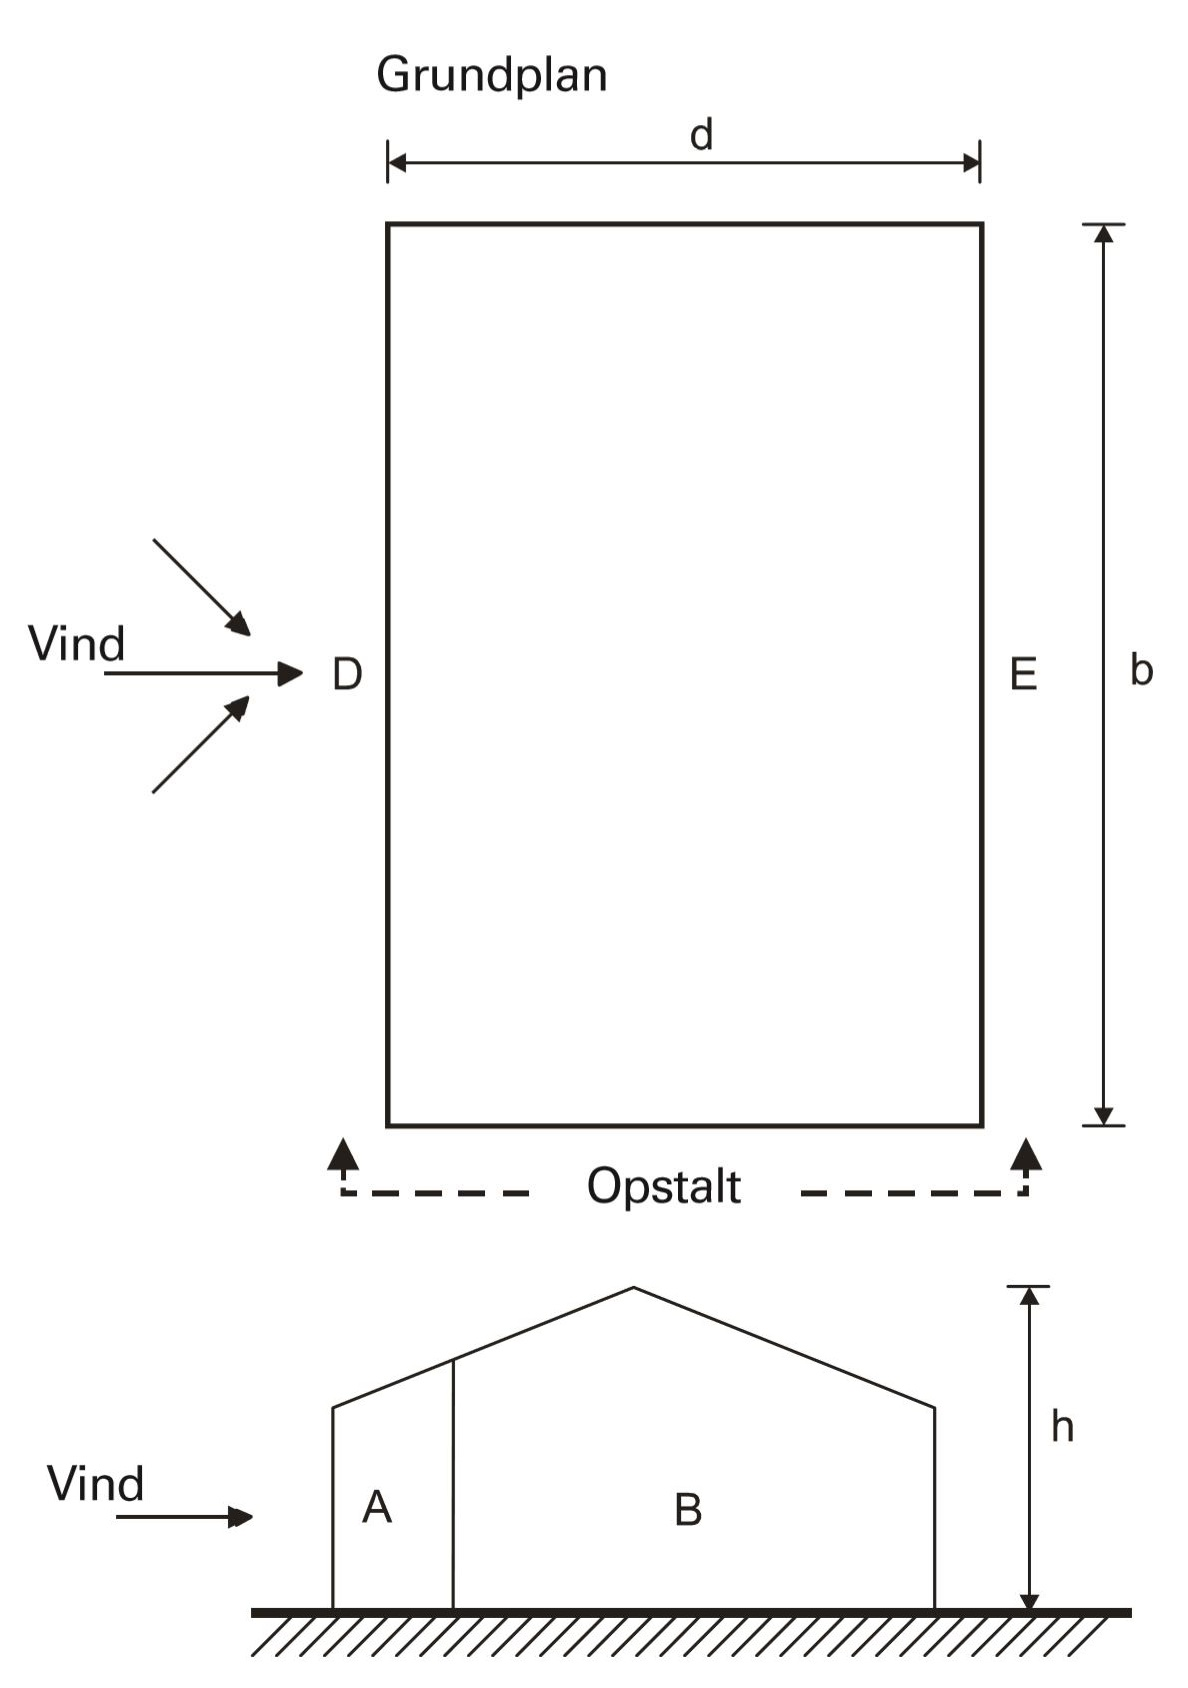
\includegraphics[width=0.60\textwidth]{billeder/Vindlast1}
\caption{Sadeltag med to forskellige skråninger og dermed to hældninger.}
\label{fig:SF1}
\end{figure}



\subsubsection{Vindlast på taget}

\begin{figure}[H] 
\centering
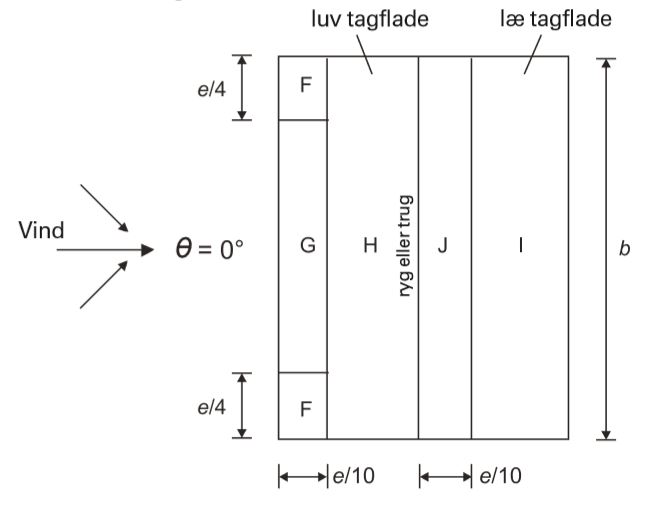
\includegraphics[width=0.60\textwidth]{billeder/Vindlast3}
\caption{Sadeltag med to forskellige skråninger og dermed to hældninger.}
\label{fig:SF1}
\end{figure}





















\section{Snelast}
Ved beregning af belastninger på en given konstruktion, så skal man også tage stilling til snelasten. Snelasten på tilbygningen regnes med formlen for vedvarende/midlertidig dimensioneringstilfælde:

$s = \mu_i \cdot C_e  \cdot  C_t \cdot s_k$

hvor

\begin{itemize}
\item $\mu_i$ = formfaktor.
\item $C_e$ = eksponeringsfaktor.
\item $C_t$ = termisk faktor
\item $s_k = karakteristisk snelast på jorden$
\end{itemize}


\subsection{Formfaktor}
Formfaktoren afhænger af tagtype og dens hældning. Tilbygningen er beklædt med et saddeltag med følgende vinkler som kan ses på figur 1: 

\begin{figure}[H] 
\centering
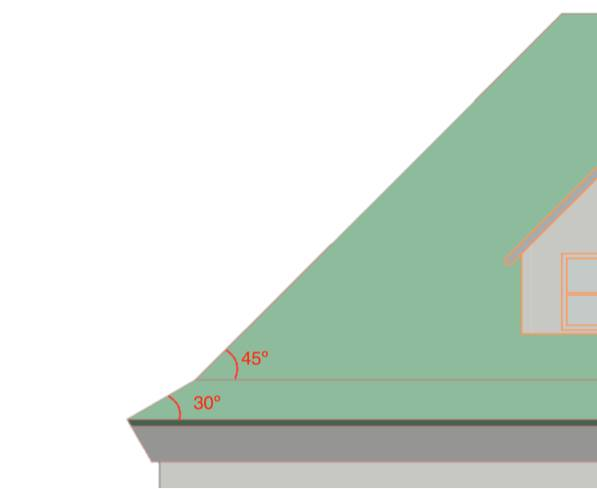
\includegraphics[width=0.60\textwidth]{billeder/SnelastFigur1}
\caption{Sadeltag med to forskellige skråninger og dermed to hældninger.}
\label{fig:SF1}
\end{figure}

Formfaktoren inddeles i tre dele; den ene med hældning på 30º, den anden med en hældning på 45º og til sidst det flade tagstykke. Form faktoren for den skrå hældning med 30º er 0,8. For den skrå hældning med 45º er værdien 0,4 og for det flade tag er værdien 0,8. 

\subsection{Eksponeringsfaktor}
Denne faktor er afhængig af omgivelserne omkring tilbygningen, men også dimensionerne på bygningen spiller en rolle. Deraf kommer formlen:

$C_e = C_{top} \cdot  C_s$

Topografien inddeles i enten vindblæst, normal eller afskærmet, alt efter hvor blottet konstruktionen. Da tilbygningen delvis er afskærmet og delvis vindblæst, så vælges der her den maksimale mulige værdi for topografien for at tage stilling til den værst mulige belastning der måtte forekomme. Værdien for topografien sættes dermed til 1,25.

Faktoren for dimensionen af konstruktionen sættes til at være lig med 1,0. Dette skyldes at den opfylder følgende sætning: $2h > l_1$, hvor $h$ svarer til højden af konstruktionen og $l_1$ svarer til den længste side af bygningen.

Eksponeringsfaktor kommer da til at få værdien på 1,25.

\subsection{Termisk faktor}
Følgende faktor bruges som en reduktionsfaktor i det tilfælde hvor der er høj varmeoverførsel såsom et drivhus med glastag. Under normale omstændigheder sættes den termisk faktor til at være 1,0.

\subsection{Karakteristisk terrænværdi}
Denne værdi sættes til at være lig med $\SI{1}{ kN/m^2}$ i Danmark

\subsection{Beregning af snelast}
De fundende faktor og variabler kan nu bruges til at finde snelasten på tilbygningen. Værdierne kan findes i tabellen forneden:

\begin{table}[H]
\centering
\begin{tabular}{|l|c|c|}
\hline
\textbf{Beskrivelse}       & \textbf{Symbol} & \textbf{Værdi}                                                                                    \\ \hline
Formfaktor                 & $\mu_i$               & \begin{tabular}[c]{@{}c@{}}0,8 (hældning 30º)\\ 0,4 (hældning 45º)\\ 0,8 (fladt tag)\end{tabular} \\ \hline
Eksponeringsfaktor         & $C_e$               & 1,25                                                                                              \\ \hline
- Topografi                & $C_{top}$               & 1,25                                                                                              \\ \hline
- Faktor for dimension     & $C_s$               & 1,0                                                                                               \\ \hline
Termisk faktor             & $C_t$               & 1,0                                                                                                 \\ \hline
Karakteristisk terrænværdi & $s_k$               & $\SI{1,0}{kN/m^2}$                                                                                              \\ \hline
\end{tabular}
\caption{Oversigt over de fundende værdier til beregning af snelast}
\label{tab:SLT1}
\end{table}


De forskellige værdier bruges til at beregne snelasten og følgende resultater kan ses i tabel \ref{tab:SLT2} Linjelasten er også beregnet over det stykke som sneen påvirket med.

\begin{table}[H]
\centering
\begin{tabular}{|l|c|c|c|}
\hline
\textbf{Tagdel}            & \textbf{Last} & \textbf{Længde} & \textbf{Linjelast} \\ \hline
Skrå del (hældning på 30º) & $\SI{1,0}{kN/m^2}$                      & 0,86 m $\cdot$ 2              & $\SI{1,73}{kN/m^2}$                                                                                                               \\ \hline
Skrå del (hældning på 45º) & $\SI{0,5}{kN/m^2}$                                     & 2,28 m $\cdot$ 2               & $\SI{4,55}{kN/m^2}$                                                                                                              \\ \hline
Fladt tag                  & $\SI{1,0}{kN/m^2}$                     &  5 m               & $\SI{5,0}{kN/m^2}$                                                                                                               \\ \hline
\end{tabular}
\caption{Oversigt over de forskellige laster for de forskellige dele som taget er blevet inddelt i.}
\label{tab:SLT2}
\end{table}


\subsection{Snelast fra sneophobning}
For bygningskonstruktioner som både udsættes for sne og vind, så regnes der med en ekstra lastarrangement. Vindsiden på sadeltaget vil have en formfaktor på nul, mens læsiden vil have en formfaktor afhængig af hældningen. Men inden der tages hensyn til den ekstra lastarrangement, så skal følgende sætninger være opfyldte:





\begin{enumerate}
\item bygningens orientering vender mod den østlige retning (fra NNØ til SØ)
\item facadehøjden i vindsiden er højst 10 m.
\item bygningens længde på tværs af vindsiden er to gange større end bygningens kiphøje
\item bygningens dybde er større end bygningens kiphøjde
\item terrænnet i vindsiden er åben i en afstand på 400 m.
\end{enumerate}

Da tilbygningen til Strøybergs Palæ opfylder alle betingelserne, så skal der regnes med ekstra last.  Igen ses der på figur 1, da de forskellige formfaktor som bruges til at udregne snelasten afhænger af hældningen på taget. For et tag med hældningen fra 15º til 30º beregnes formfaktoren til at være lig med 1,2. Derimod beregnes formfaktoren til at være 0,60 for taget med hældningen 45º. 

Til beregning af den ekstra snelast bruges den samme formel som tidligere anvendt i starten af kapitlet. Igen bruges denne formel til at beregne den ekstra snelast, formfaktoren er blot ændret:

$s = \mu_i \cdot C_e  \cdot  C_t \cdot s_k$

Resultatet kan ses i tabel \ref{tab:SLT3} hvor linjelasten også er skrevet ind.

\begin{table}[H]
\centering
\begin{tabular}{|l|c|c|c|}
\hline
\textbf{Tagdel}            & \textbf{Last} & \textbf{Længde} & \textbf{Linjelast} \\ \hline
Skrå del (hældning på 30º) & $\SI{0,75}{kN/m^2}$                      & 0,86 m $\cdot$ 2              & $\SI{2,59}{kN/m^2}$                                                                                                               \\ \hline
Skrå del (hældning på 45º) & $\SI{0,5}{kN/m^2}$                                     & 2,28 m $\cdot$ 2               & $\SI{6,82}{kN/m^2}$                                                                                                              \\ \hline
\end{tabular}
\caption{Oversigt over de ekstra snelaster der fremkommer ved låsiden ved vindblæst.}
\label{tab:SLT3}
\end{table}
















\chapter{Snelast}
Ved beregning af belastninger på en given konstruktion, så skal man også tage stilling til snelasten. Snelasten på tilbygningen regnes med formlen for vedvarende/midlertidig dimensioneringstilfælde:

$s = \mu_i \cdot C_e  \cdot  C_t \cdot s_k$

hvor

\begin{itemize}
\item $\mu_i$ = formfaktor.
\item $C_e$ = eksponeringsfaktor.
\item $C_t$ = termisk faktor
\item $s_k = karakteristisk snelast på jorden$
\end{itemize}


\section{Formfaktor}
Formfaktoren afhænger af tagtype og dens hældning. Tilbygningen er beklædt med et saddeltag med følgende vinkler som kan ses på figur 1: 

\begin{figure}[H] 
\centering
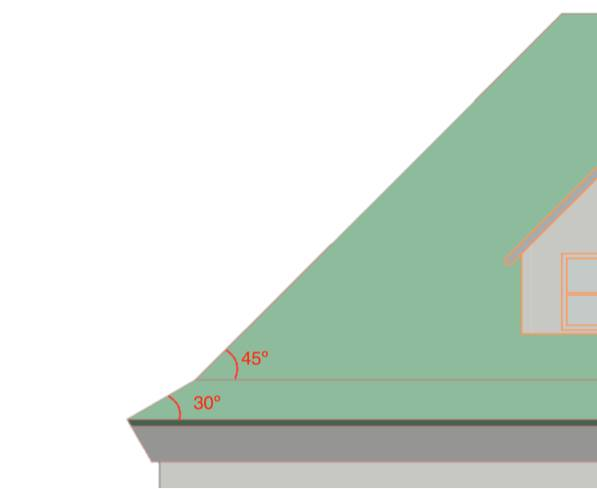
\includegraphics[width=0.60\textwidth]{billeder/SnelastFigur1}
\caption{Sadeltag med to forskellige skråninger og dermed to hældninger.}
\label{fig:SF1}
\end{figure}

Formfaktoren inddeles i tre dele; den ene med hældning på 30º, den anden med en hældning på 45º og til sidst det flade tagstykke. Form faktoren for den skrå hældning med 30º er 0,8. For den skrå hældning med 45º er værdien 0,4 og for det flade tag er værdien 0,8. 

\section{Eksponeringsfaktor}
Denne faktor er afhængig af omgivelserne omkring tilbygningen, men også dimensionerne på bygningen spiller en rolle. Deraf kommer formlen:

$C_e = C_{top} \cdot  C_s$

Topografien inddeles i enten vindblæst, normal eller afskærmet, alt efter hvor blottet konstruktionen. Da tilbygningen delvis er afskærmet og delvis vindblæst, så vælges der her den maksimale mulige værdi for topografien for at tage stilling til den værst mulige belastning der måtte forekomme. Værdien for topografien sættes dermed til 1,25.

Faktoren for dimensionen af konstruktionen sættes til at være lig med 1,0. Dette skyldes at den opfylder følgende sætning: $2h > l_1$, hvor $h$ svarer til højden af konstruktionen og $l_1$ svarer til den længste side af bygningen.

Eksponeringsfaktor kommer da til at få værdien på 1,25.

\section{Termisk faktor}
Følgende faktor bruges som en reduktionsfaktor i det tilfælde hvor der er høj varmeoverførsel såsom et drivhus med glastag. Under normale omstændigheder sættes den termisk faktor til at være 1,0.

\section{Karakteristisk terrænværdi}
Denne værdi sættes til at være lig med $\SI{1}{ kN/m^2}$ i Danmark

\section{Beregning af snelast}
De fundende faktor og variabler kan nu bruges til at finde snelasten på tilbygningen. Værdierne kan findes i tabellen forneden:

\begin{table}[H]
\centering
\begin{tabular}{|l|c|c|}
\hline
\textbf{Beskrivelse}       & \textbf{Symbol} & \textbf{Værdi}                                                                                    \\ \hline
Formfaktor                 & $\mu_i$               & \begin{tabular}[c]{@{}c@{}}0,8 (hældning 30º)\\ 0,4 (hældning 45º)\\ 0,8 (fladt tag)\end{tabular} \\ \hline
Eksponeringsfaktor         & $C_e$               & 1,25                                                                                              \\ \hline
- Topografi                & $C_{top}$               & 1,25                                                                                              \\ \hline
- Faktor for dimension     & $C_s$               & 1,0                                                                                               \\ \hline
Termisk faktor             & $C_t$               & 1,0                                                                                                 \\ \hline
Karakteristisk terrænværdi & $s_k$               & $\SI{1,0}{kN/m^2}$                                                                                              \\ \hline
\end{tabular}
\caption{Oversigt over de fundende værdier til beregning af snelast}
\label{tab:SLT1}
\end{table}


De forskellige værdier bruges til at beregne snelasten og følgende resultater kan ses i tabel \ref{tab:SLT2} Linjelasten er også beregnet over det stykke som sneen påvirket med.

\begin{table}[H]
\centering
\begin{tabular}{|l|c|c|c|}
\hline
\textbf{Tagdel}            & \textbf{Last} & \textbf{Længde} & \textbf{Linjelast} \\ \hline
Skrå del (hældning på 30º) & $\SI{1,0}{kN/m^2}$                      & 0,86 m $\cdot$ 2              & $\SI{1,73}{kN/m^2}$                                                                                                               \\ \hline
Skrå del (hældning på 45º) & $\SI{0,5}{kN/m^2}$                                     & 2,28 m $\cdot$ 2               & $\SI{4,55}{kN/m^2}$                                                                                                              \\ \hline
Fladt tag                  & $\SI{1,0}{kN/m^2}$                     &  5 m               & $\SI{5,0}{kN/m^2}$                                                                                                               \\ \hline
\end{tabular}
\caption{Oversigt over de forskellige laster for de forskellige dele som taget er blevet inddelt i.}
\label{tab:SLT2}
\end{table}


\section{Snelast fra sneophobning}
For bygningskonstruktioner som både udsættes for sne og vind, så regnes der med en ekstra lastarrangement. Vindsiden på sadeltaget vil have en formfaktor på nul, mens læsiden vil have en formfaktor afhængig af hældningen. Men inden der tages hensyn til den ekstra lastarrangement, så skal følgende sætninger være opfyldte:





\begin{enumerate}
\item bygningens orientering vender mod den østlige retning (fra NNØ til SØ)
\item facadehøjden i vindsiden er højst 10 m.
\item bygningens længde på tværs af vindsiden er to gange større end bygningens kiphøje
\item bygningens dybde er større end bygningens kiphøjde
\item terrænnet i vindsiden er åben i en afstand på 400 m.
\end{enumerate}

Da tilbygningen til Strøybergs Palæ opfylder alle betingelserne, så skal der regnes med ekstra last.  Igen ses der på figur 1, da de forskellige formfaktor som bruges til at udregne snelasten afhænger af hældningen på taget. For et tag med hældningen fra 15º til 30º beregnes formfaktoren til at være lig med 1,2. Derimod beregnes formfaktoren til at være 0,60 for taget med hældningen 45º. 

Til beregning af den ekstra snelast bruges den samme formel som tidligere anvendt i starten af kapitlet. Igen bruges denne formel til at beregne den ekstra snelast, formfaktoren er blot ændret:

$s = \mu_i \cdot C_e  \cdot  C_t \cdot s_k$

Resultatet kan ses i tabel \ref{tab:SLT3} hvor linjelasten også er skrevet ind.

\begin{table}[H]
\centering
\begin{tabular}{|l|c|c|c|}
\hline
\textbf{Tagdel}            & \textbf{Last} & \textbf{Længde} & \textbf{Linjelast} \\ \hline
Skrå del (hældning på 30º) & $\SI{0,75}{kN/m^2}$                      & 0,86 m $\cdot$ 2              & $\SI{2,59}{kN/m^2}$                                                                                                               \\ \hline
Skrå del (hældning på 45º) & $\SI{0,5}{kN/m^2}$                                     & 2,28 m $\cdot$ 2               & $\SI{6,82}{kN/m^2}$                                                                                                              \\ \hline
\end{tabular}
\caption{Oversigt over de ekstra snelaster der fremkommer ved låsiden ved vindblæst.}
\label{tab:SLT3}
\end{table}





%\chapter{Konklusion}
Denne rapport dokumenterer, at den nordlige gangbro ved KMD er konstrueret korrekt i form af tilstrækkelig bæreevne i forhold til de forskellige laster, som den bliver udsat for. 

Ud fra rapporten konkluderes der, at KMDs gangbro er en konstruktion, der er konstrueret som en gitterkonstruktion. En gitterkonstruktion er en konstruktion, som er opbygget af stænger, som udgør trekanter. Konstruktionen er opbygget som en statisk ubestemt konstruktion, men for at gøre det muligt at beregne de indre kræfter, ved hjælp af knudepunktsmetoden i konstruktionen, er der indsat en fiktiv stang for at gøre konstruktionen statisk bestemt.  

Stål er et velegnet materiale til gangbroen, da stål har en meget høj trækstyrke, hvilket underflangen af gangbroen vil blive udsat for. En anden grund til, at stål er et velegnet byggemateriale er, at det kan fremstilles i en lang række forskellige kvaliteter, alt efter hvilken opgave det skal have.

I denne rapport er der blevet beregnet på fire forskellige laster, som påvirker KMDs gangbro; egen-, nytte-, vind- og snelast. De forskellige laster er blevet ført ud på 48 forskellige knudepunkter. Egenlasten er den last, som en konstruktion belaster sig selv med og er blevet beregnet ud fra de materialer gangbroen er bygget af. Nyttelasten er den last, som gangbroen udsættes for af mennesker og inventar. Nyttelasten er beregnet ud fra en standard, som passer til gangbroens kategori i forhold til hvad den anvendes til. Vindlast er den last, som vinden påvirker en konstruktion med. Vindlasten er beregnet ud fra en række standarder og normer, fundet i Eurocodes, såsom hvor høj en konstruktion er, hvilket område konstruktionen ligger i, om der står andre konstruktioner i nærheden og hvor i landet konstruktionen ligger. Vindlasten er den eneste last, der i denne rapport både påvirker det vertikale og horisontale gitter. Snelasten er den last, som sne påvirker en konstruktion med, den virker udelukkende på taget af KMDs gangbro og den kan både være jævnt og ujævnt fordelt derpå. Snelasten beregnes også ud fra information, der fås i Eurocode og ud fra, at der forekommer snedriver når konstruktionen ligger imellem to højere konstruktioner, som er tilfældet for KMDs gangbro. 

Ud fra egen-, nytte-, vind- og snelasterne er der blevet beregnet lastkombinationer hvor de forskellige laster på skift er beregnet som dominerende. Der bliver ganget partialkoefficienter på lastkombinationerne for at sørge for, at lasterne bliver overvurderet i forhold til hvor store de er i den virkelige verden. Dette gøres for at sikre en mindre risiko for kollaps, da modeller og virkelighed ikke altid stemmer overens. Laster hvor partialkoefficienter er multipliceret på kaldes regningsmæssige laster. Den største regningsmæssige last bliver herefter anvendt til eftervisning af bæreevnen. På KMDs gangbro er det den lastkombination, hvor nyttelasten er dominerende, der er størst. 


Med viden om, at gangbroen er statisk bestemt, er stangkræfterne beregnet ved anvendelse af knudepunktsmetoden. Ved brug af knudepunktsmetoden løsskæres alle knudepunkter fra hinanden og der beregnes horisontal og vertikal ligevægt for indre kræfter ved knudepunkter.  Ved beregningerne af stangkræfterne bliver det fastlagt hvilke stænger der er træk- eller trykstænger. Ud fra de beregnede indre kræfter, er der opstillet en statisk model, som efterviser, at den regningsmæssige spænding er lavere end profilens maksimale tilladte spænding.  

Ud fra den statiske dokumentation kan det konkluderes, at de regningsmæssige spændinger i profilerne er mindre end den tilladte spænding, derfor er gangbroen dimensioneret tilstrækkeligt, ud fra de antagelser der er lavet i rapporten. Den fiktive stang der blev placeret for at kunne anvende knudepunktsmetoden, og ud fra beregningen af de indre kræfter kan det konkluderes, at den fiktive stang er minimalt belastet.  

 



%%%% Kilder %%%%


\begingroup
	\raggedright
	\bibliography{bibtex/mybib.bib}						% Litteraturlisten inkluderes
\endgroup

%%%% Fixme-listen %%%%

\newpage														% Ny side til Fixme-listen
%\listoffixmes													% Fixme-listen - fjernes til sidst i projektet med "%"


%%%% Appendiks %%%%

\appendix
\clearforchapter												% Sikrer at pagestylen aktiveres paa den rigtige side
\phantomsection													% Kunstigt afsnit, som hyperlinks kan 'holde fast i'
\pdfbookmark[0]{Appendiks}{appendiks}							% Tildeler en klikbar bookmark til den endelige PDF

%% Indstillinger for appendiks (deaktiveret med "%") %%

%\pagestyle{empty}												% Sidehoved/-fod for standardsider aendres til tom for appendiks
%\aliaspagestyle{chapter}{empty}								% Sidehoved/-fod for kapitelsider aendres til tom for appendiks
%\settocdepth{chapter}											% Kun kapitel-niveau vises i ToC
%\addtocontents{toc}{\protect\cftpagenumbersoff{chapter}}		% Sidetal for kapitler fjernes i ToC

%% Filer til appendiks %%

														% Appendiks/bilag start - giver chapter bogstaver i stedet for tal
%\input{appendiks/appendiks2}
%%%% Bilag %%%%

%\phantomsection												% Kunstigt afsnit, som hyperlinks kan 'holde fast i'
%\addcontentsline{toc}{chapter}{Bilag A \ Navn} 				% Manuelle indgange i indholdsfortegnelsen (naar \includepdf bruges)

%\includepdf[pages={x-y}]{filnavn}								% Inkluder eksterne bilag med \includepdf[pages={x-y}]{filnavn}


\end{document}													% Slutter dokumentet - obligatorisk
